\documentclass[12pt,oneside]{book}

\usepackage[dvips,letterpaper,margin=0.75in,bottom=0.75in]{geometry}
\usepackage{cite}
\usepackage{slashed}
\usepackage{graphicx}
\usepackage{amsmath}
\usepackage{enumitem}
\usepackage{amsthm}
\usepackage{braket}
\usepackage{listings}
\theoremstyle{definition}

\usepackage[american,fulldiode]{circuitikz}
\tikzset{component/.style={draw,thick,circle,fill=white,minimum size =0.75cm,inner sep=0pt}}
\newtheorem{measurement}{Logbook Entry}[chapter]
\newtheorem{plot}{Jupyter Notebook}[chapter]

\begin{document}
\ctikzset{bipoles/thickness=1}
\ctikzset{bipoles/length=.6cm}

\title{Physics 40 Lab Manual}
\author{Michael Mulhearn}
\maketitle

\tableofcontents

\chapter{Installation of Scientific Python}

\section{Introduction}

In this lab, you will install the software which we will be using in
phy40. This is an assignment, and will be graded.  You should submit a
text file containing a log of all the steps you took to install the
software on your computer.  Make this log as specific as possible, an
entry might be:
\begin{verbatim}
Downloaded windows installer from:
 https://repo.anaconda.com/miniconda/Miniconda3-latest-Windows-x86_64.exe
\end{verbatim}  
Keeping this log will also make it easier for you to get help if you
have problems.

If you run into problems, do some research on a web search tool
(Google, for example) to become better informed and to see if you can
overcome the problem on your own before asking for help.  This is an
important technique in getting help with technical problems that will
serve you well even outside of this class.  You will find it more easy
to get useful technical help, from the sort of people most capable of
offering it, when it is clear from your question that you are informed
and have already tried all of the obvious things.  If you are still
stuck after trying to solve the problem for yourself, then contact
your TA or instructor with specific technical details about what is
failing, and include your installation log.

If you do find a problem with these instructions or manage to overcome
a technical problem yourself, make sure to note it in your log and
inform your TA, in case it is helpful for other students.

\section{Installing Miniconda3}

We will be using Miniconda3 based on Python 3.7 for data analysis
using Jupyter notebooks.  Miniconda is a lightweight package which we
can use to install all of the remaining analysis software we will need
in a consistent manner across all different operating systems.

Determine which OS type and version you have on the desktop or laptop
computer that you will be using for your coursework.  The software
here will work under Windows, Linux, or macOS.  It should also work on
all Chromebooks released since 2019, and some earlier Chromebooks.
You should also check whether you have a 32-bit or 64-bit OS (you can
find instructions for how to determine this for your particular OS
version with a Google search.)  Most desktop or laptop computers built
in the last ten years are 64-bit.

If you are using Linux or macOS, then from within a terminal type:
\begin{lstlisting}{language=csh}
 echo $SHELL
\end{lstlisting}
to determine the shell you are using (typically "bash" these days).
Record all of this information in your installation log file.

Once you have determined your OS type and version, follow the
instructions below approprate to your operating system.

\subsection{Installing under Windows}

If you have already installed a version of conda (e.g. Anaconda or
Miniconda) then you do not need to re-install it.  Instead, find the
the Anaconda Prompt in the Application menu and run it.

If you need to install Miniconda3, then download and run the
appropriate installer from:
\begin{verbatim}
https://docs.conda.io/en/latest/miniconda.html#
\end{verbatim}
If prompted, you should choose to:
\begin{itemize}
 \item Accept the license / terms of use.
 \item Install for just the current user, not all users.
\end{itemize}
 Once installed, check that you can run the "Anaconda Prompt". From
the prompt, check that you can run:
\begin{lstlisting}{language=csh}
  conda --version
\end{lstlisting}
and note the output in your installation log.  Then proceed to
Section~\ref{sec:env}.

\subsection{Installing on a Chromebook}

You will need to activate Linux on your Chromebook, according to the instructions here:

\begin{verbatim}
https://www.codecademy.com/articles/programming-locally-on-chromebook
\end{verbatim}

Then follow the insturctions for installing under Linux.  If your
Chromebook predates 2019 and does not support Linux, contact your
instructor for alternative arrangements.

\subsection{Installing Miniconda3 under Linux or macOS}

If you believe you already already have a version of conda installed
(such as miniconda or ananconda) , check by running
\begin{lstlisting}{language=csh}
   conda --version
\end{lstlisting}
If you see something like:
\begin{lstlisting}{language=csh}
  conda 4.9.2
\end{lstlisting}
as output (even if the version is different) then you do indeed already have conda
installed, with the base environment activated, and you can skip ahead to
Section~\ref{sec:env}.  If instead you get a message like:
\begin{lstlisting}{language=csh}
   conda: command not found
\end{lstlisting}
then the easiest solution is to simply proceed with these instructions.

To install Miniconda, download the appropriate installer for your OS
here:
\begin{verbatim}
  https://docs.conda.io/en/latest/miniconda.html\#
\end{verbatim}
For macOS, you can choose between a "package" or "bash" version. I
find it easier to follow the bash version, but the package version
will work too. I recommend you make the following choices if prompted:
\begin{itemize}
\item Accept the license / terms of use.
\item Do not install for all users, but just one the current user.
\item Do allow the installer to issue ``conda init''.
\end{itemize}
During the installation, take note of the install location in your log.

After installation with these settings, conda will automatically
activate the ``base'' conda environment.  If this annoys you, as it
does me, or interferes with other software you are using, you can turn
off this agressive behavior with:
\begin{lstlisting}{language=csh}
   conda config --set auto_activate_base false
\end{lstlisting}

Confirm that you have successfully installed conda by typing
\begin{lstlisting}{language=csh}
   conda --version
\end{lstlisting}
Record the output in your installation log, and proceed to Section~\ref{sec:env}.

\section{Installing the Physics 40 Conda Environment}
\label{sec:env}

Make sure your conda is fully up to date with:
\begin{lstlisting}{language=csh}
  conda update conda
\end{lstlisting}
Then follow the prompts, e.g. selecting "y" as needed to update any out-of-date packages.

We'll be using a conda environment specifically for phy40 to avoid
conflicts with any other projects on your computer, and to ensure that
we all have the same software installed.  To create our environment:
\begin{lstlisting}{language=csh}
  conda create -n phy40 python=3.9 numpy scipy matplotlib ipython jupyter
\end{lstlisting}
  
\section{Starting a Jupyter notebook}

This course will make extensive use of the Jupyter Notebook interface
to Scientific Python, which is well suited to academic work (including
independent research) because it combines code with output in
digestable chunks.  Even when the end product is a polished peice of
software, much of the initial code development can be done in the interactive
session that Jupyter Notebooks provide.  

\begin{figure}[htbp]
\begin{center}
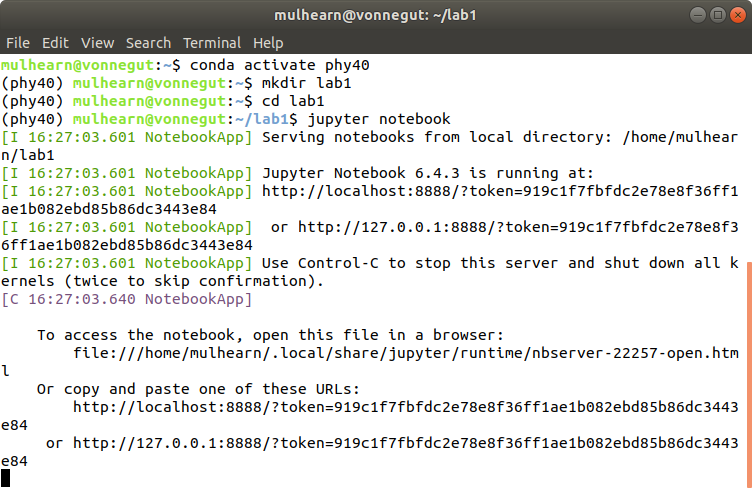
\includegraphics[width=0.65\textwidth]{figs/install/jupyter_startup.png} 
\caption{Example starting Jupyter Notebook from the Linux command line.  In Windows, you will need to open the Anaconda Prompt instead of a terminal.}
\label{fig:jupyterstartup}
\end{center}
\end{figure}

\begin{figure}[htbp]
\begin{center}
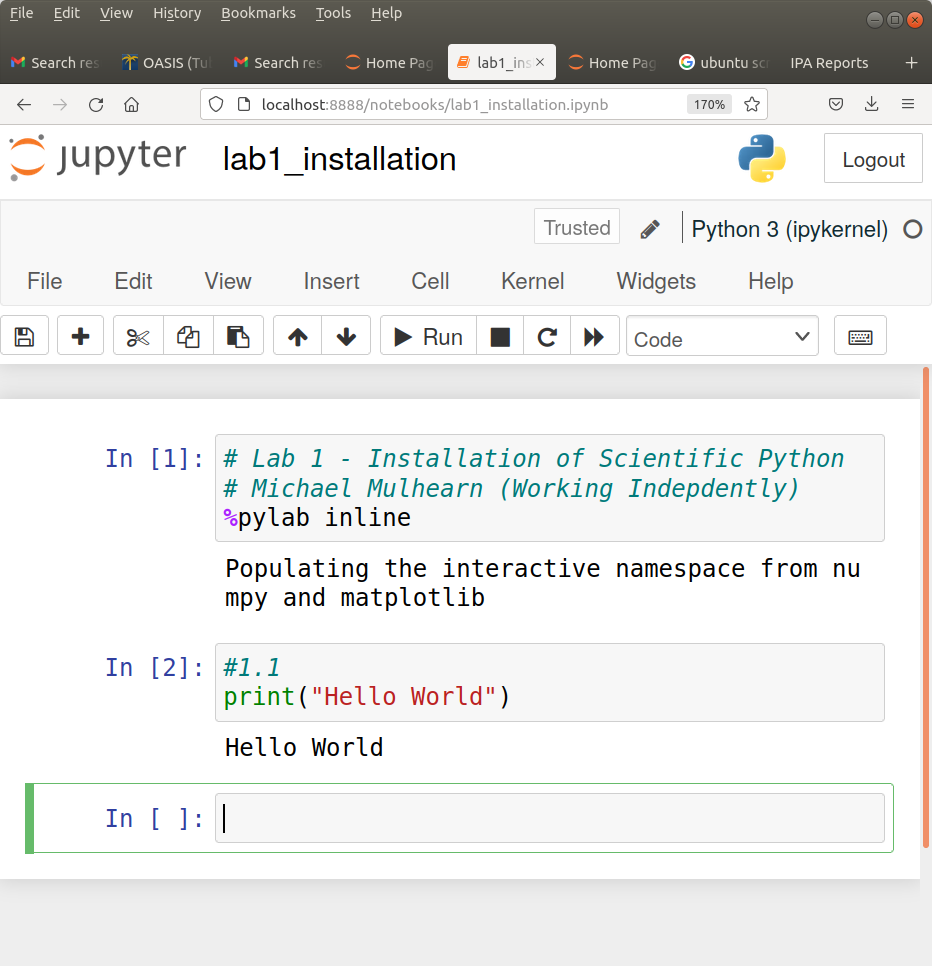
\includegraphics[width=0.65\textwidth]{figs/install/jupyter_window.png} 
\caption{The Hello World example Jupyter Notebook.}
\label{fig:jupyterwindow}
\end{center}
\end{figure}

\begin{figure}[htbp]
\begin{center}
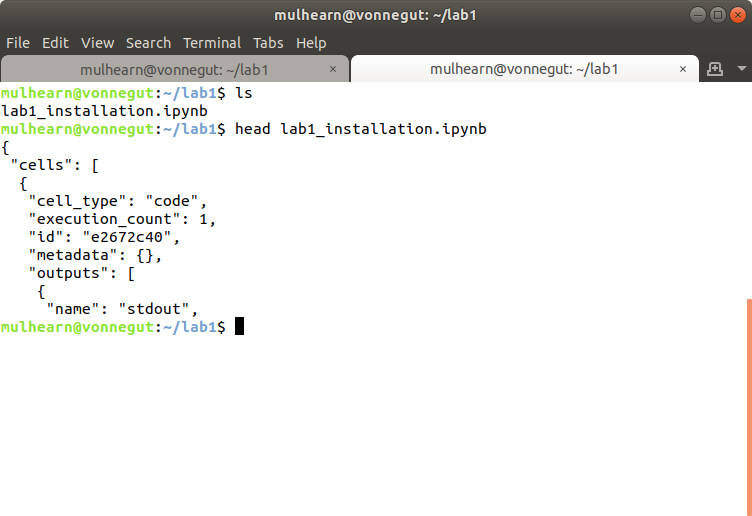
\includegraphics[width=0.65\textwidth]{figs/install/jupyter_saved.png} 
\caption{Example showing the saved Jupyter notebook.  Notice that notebook file (ipynb) is not human readable on its own: it requires the Jupyter software to render it in a human readable form.}
\label{fig:jupytersaved}
\end{center}
\end{figure}

To activate the phy40 environment type:
\begin{lstlisting}{language=csh}
  conda activate phy40
\end{lstlisting}
When you are done with Phy 40 for the day you can deactivate this
environment (later) with:
\begin{lstlisting}
  conda deactivate
\end{lstlisting}
Launch jupyter notebook with:
\begin{lstlisting}
  jupyter notebook
\end{lstlisting}
This should start the Jupyter Notebook server and open a client in your web browser.
An example starting a Jupyter Notebook from Linux is shown in Fig.~\ref{fig:jupyterstartup}.

You should create one Jupyter Notebook per lab assignment, by choosing
the New (Python 3) option in your client.  Change the name of your
notebook to something that clearly identifies the lab.  Start each lab
with comments (starting with ``\#'' symbol) indicating the title of
the lab, then your name followed by your lab partners.  See the first
cell of Fig.~\ref{fig:jupyterwindow} for an example.  This first cell
is also a good place to issue the ipython ``magic function'':
\begin{verbatim}
%pylab inline
\end{verbatim}
which will setup the notebook for inline plots and load the numpy and matplotlib libraries for you.

Each assignment will consist of a number of steps, clearly numbered like this one, your first step:\\

\plot Print ``hello world'' using the python print command.\\

\noindent
To keep your notebook clear, label cells (such as this one) with a
comment for the assignment step number, as in the second cell of
Fig.~\ref{fig:jupyterwindow}.  You only need to label one cell if the
assignment is fullfilled across several cells.

Jupyter Notebook checkpoints your work automatically.  You should be
able to see your notebook saved in the working directory where you
started, as in Fig.~\ref{fig:jupytersaved}.  Notice that while the
notebook file is ASCII text, it is not a human readable format.  The
Jupyter software is needed to render the notebook in a human readable
way.  To make your grader's life easier, you will be submitting PDF
versions of your notebook, once all of the tasks are completed and the
output is visible.  There are several ways to make a PDF file from
your notebook, but the most reliable is to use the ``Print Preview''
option to view the notebook as a PDF file within your browser, then
use the print feature of your browser to print the page as a PDF file.
Try this now, and make sure you can create a legible PDF file, but do
not submit it to the course site, as you still have more to do.
Always keep your python notebook file (ipynb) even after you submit
the assignment.  If you have problems, you can reproduce a PDF file
from the notebook file, but it is tedious to reproduce your notebook
from PDF.  If you have problems producing the PDF file, you can submit
the ``ipynb'' file as a temporary work-around, but work with your TA
to sort out the problem as quickly as possible.

\section{Submitting your assignment}

Before submitting, take some time to clean up your assignments to
remove anything superfluous and place the exercises in the correct
order.  You can also add comments as needed to make your work clear.
You can use the Cell $\to$ All Output $\to$ Clear and Cell $\to$ Run
All commands to make sure that all your output is up to date with the
cell source.

When you are satisfied with your work, print the PDF file as described
earlier and submit it to the course website.










%\chapter{Introduction to Plotting}

\section{Introduction}
This exercise will introduce calculations and plotting techniques using
numpy arrays within Scientific Python.

\section{Plotting discrete data and continuous functions}

\begin{figure}[htbp]
\begin{center}
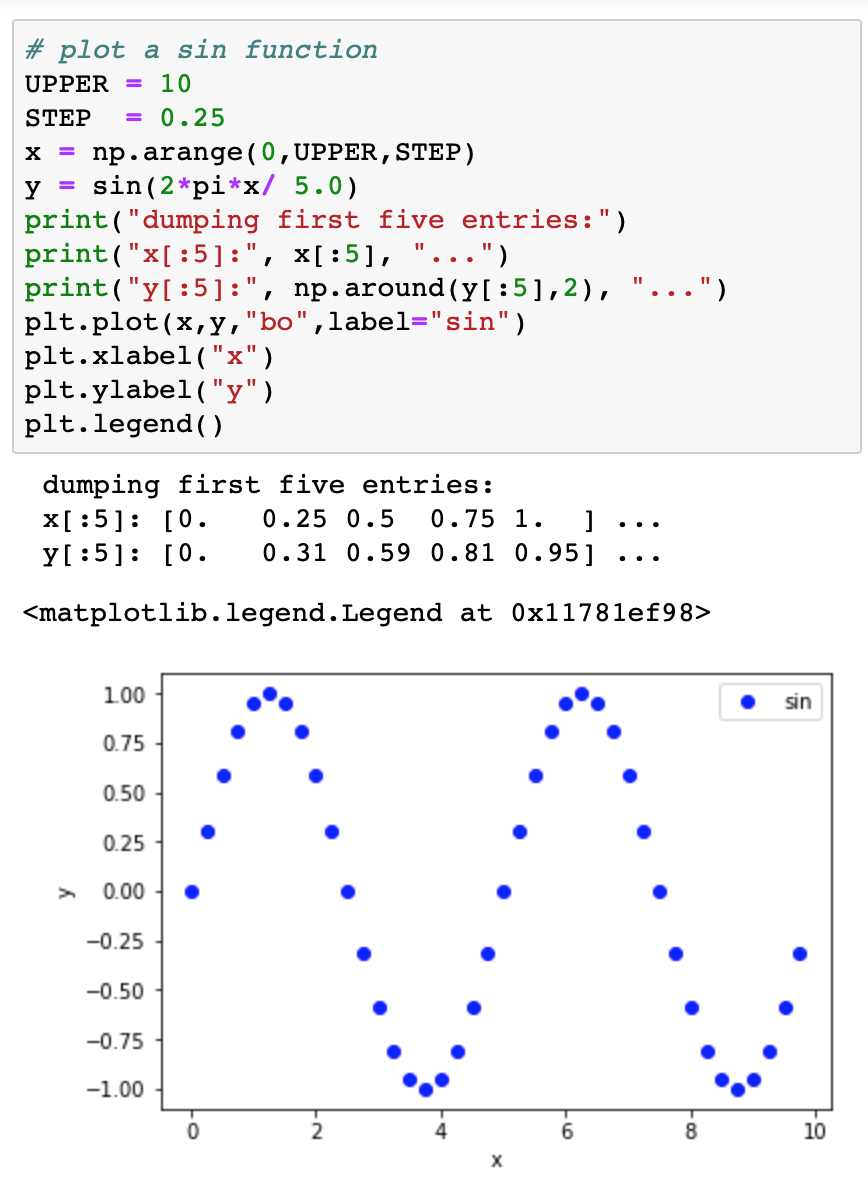
\includegraphics[width=0.65\textwidth]{figs//plotting/plotting.png} 
\caption{Circuit for verifying Ohm's law as a (a) circuit diagram, and (b) implemented using your lab equipment.}
\label{fig:plotsin}
\end{center}
\end{figure}

Consider the Jupyter notebook example in Fig.~\ref{fig:plotsin} which
plots a sine function sampled at discrete values.  Note the following
key features, which you will use repeatedly today and in future labs:
\begin{itemize}
\item Use of global variables {\tt UPPER} and {\tt STEP} at the top of
  the snippet, allowing for easy adjustment of parameters that affect
  the plot.
\item Use of {\tt np.arange} to define an array of x values.
\item Creation of the array y, defined by $y = \sin(2\pi x / 5)$ for each value of x.  One of the great joys of using numpy is the ability to avoid getting bogged down with explicit for loops.
\item Use of slicing techniques {\tt x[:5]} to show only the first five entries for debugging.  
\item Plotting the arrays of $x$ and $y$ values with {\tt plt.plot}  using the {\tt "bo"} option for blue circles.
\item Defining appropriate axis labels with {\tt plt.xlabel} and {\tt plt.xlabel}. 
\item Creation of a legend using the {\tt label} option to {\tt plt.plot} and the {plot.legend()} command.
\end{itemize}
Notice that even in this simple example, I've added some intermediate
feedback from my code in the form of the screen dumps of the first few
values of $x$ and $y$.  It's a common pitfall to try and rush ahead to
the final product when programming.  But it is much faster and
reliable to break your task into small steps, and establish feedback
at each small step.  To plot a continuous function with Scientific
Python, you will still use discrete data but:

\begin{itemize}
 \item Use much finer binning of the $x$-axis variable to draw a smooth curve. 
 \item Use the line option {\tt "-"} or dashed line {\tt "--"} instead of points with {\tt "o"}. 
\end{itemize} 

\noindent
{\bf Plot 1:}  Plot the quadratic function $y = x^2$ with the following requirements:
\begin{itemize}
 \item Plot in the range $x = [0,20)$.
 \item Plot discrete samples with a step size of $2$ using blue circles.
 \item On the same axis, plot the corresponding smooth function using a red solid line.
 \item Add appropriate axis labels. 
 \item Add a legend for the ``discrete'' and the ``smooth''  function.
\end{itemize}

\section{Multivariate analysis using boolean masks}
\begin{figure}[htbp]
\begin{center}
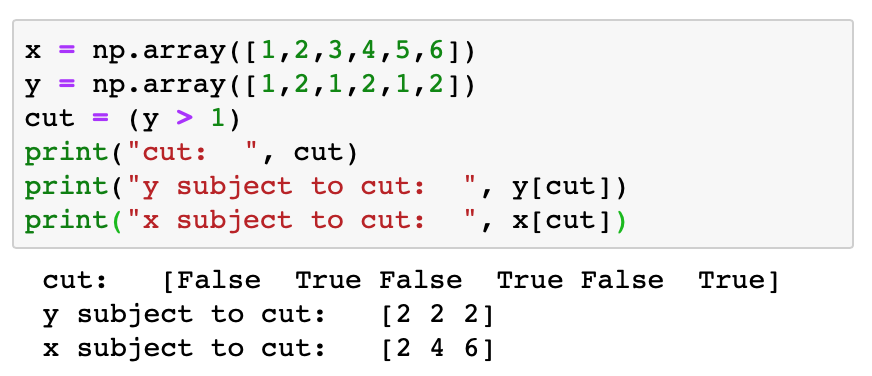
\includegraphics[width=0.65\textwidth]{figs//plotting/booleanmasks.png} 
\caption{Using boolean masks to cut on variable $y$.}
\label{fig:booleanmasks}
\end{center}
\end{figure}

A powerful technique in Scientific Python for performing analysis involving multiple variables uses boolean masks as shown in Fig.~\ref{fig:booleanmasks}.  In the example:
\begin{itemize}
\item Two numpy arrays $x$ and $y$ {\tt of the same length} are defined to contain the collected data.
\item The cut defined by $y > 1$ is a boolean array of the same length as $x$ and $y$ which is true at indices where the condition is met and false where it is not.
\item The subset of the entire $y$ array defined by {\tt y[cut]} consists only of those entries of $y$ for which the condition $y>1$ is met.
\item The subset of the entire $x$ array defined by {\tt x[cut]} consists only of those entries of $x$ for which the condition $y>1$ is met for the corresponding y value.
\end{itemize}
The last item shows the real power of this technique, one can look at one variable subject to constraints on another variable.

\begin{table}
\caption{Sample data for a voltage measurement subject to high frequency noise.}
\label{tbl:hfnoiseeg}
\begin{center}
\begin{tabular}{lll}
$t~(\rm s)$ & $v~(\rm V)$ & $n$ \\
0.4  & 0.25  &  2.8 \\
1.1  & 2.37  &  7.3 \\
1.4  & 1.69  &  9.7 \\
1.9  & 0.93  &  1.3 \\
2.5  & -1.0  &  6.2 \\
3.0  & 0.95  &  4.8 \\
3.4  & 1.22  &  6.9 \\
4.1  & 0.54  &  4.0 \\
4.4  & 0.37  &  1.9 \\
4.8  & 0.13  &  4.0 \\
5.5  & -2.04  &  9.5 \\
6.2  & -2.06  &  8.7 \\
6.5  & -0.81  &  2.3 \\
7.0  & -0.95  &  5.3 \\
7.5  & 0.98  &  9.7 \\
7.9  & 0.27  &  8.3 \\
8.5  & -0.81  &  0.1 \\
9.0  & -0.59  &  5.1 \\
9.4  & -0.37  &  4.4 \\
9.9  & 0.56  &  9.9 \\
\end{tabular}
\end{center}
\end{table}

Next consider the sample data in Table~\ref{tbl:hfnoiseeg} which comes from experimental measurements of a voltage level $v$ at discrete times $t$.  The measurement is subject to a high-frequency noise monitoring by the variable $n$.  The noise is only present for $n > 6.0$.  A straightforward way to load this data into scientific python is by defining numpy arrays for each variable as follows:
\begin{verbatim}
t = np.array([0.4, 1.1, 1.4, 1.9, 2.5, 3.0, 3.4, 4.1, 4.4, 4.8, 
                     5.5, 6.2, 6.5, 7.0, 7.5, 7.9, 8.5, 9.0, 9.4, 9.9])
v = np.array([ 0.25, 2.37, 1.69, 0.93, -1.0, 0.95, 1.22,   
                      0.54, 0.37, 0.13, -2.04, -2.06, -0.81, -0.95,  
                      0.98, 0.27, -0.81, -0.59, -0.37, 0.56])
n = np.array([2.8, 7.3, 9.7, 1.3, 6.2, 4.8, 6.9, 4.0, 1.9, 4.0,  
                      9.5, 8.7, 2.3, 5.3, 9.7, 8.3, 0.1, 5.1, 4.4, 9.9])
\end{verbatim}

\noindent
{\bf Plot 2} Prepare a plot of the sample data subject to the following:
\begin{itemize}
 \item Plot the voltage as a function of time as discrete data using red points.
 \item Define the boolean array {\tt keep} based on the noise reducing condition $n<=6.0$.
 \item Plot the voltage as a function of time, subject to the noise reducing condition using blue points.
 \item Plot the function $\sin(2 \pi x / 10)$ as a smooth function.
 \item Add appropriate axis labels.
 \item Add a legend for ``raw'' data with no cut, ``clean'' data with noise removed, and your continuous ``sin'' function.   
\end{itemize}
Your plot will reveal a clear sine function in the discrete data (after noise removal) consistent with the continuous function.  





%\chapter{The Monte Carlo Method}

\section{Introduction}

This lab, which will take two lab sessions to complete, introduces the
Monte Carlo method, an approach to solving a wide range of problems by
repeatedly drawing random numbers from a probability distribution.
You will produce a sequence of pseudorandom numbers.  You will use a
histogram to directly compare values of random variables to a
probability distribution function.  With these preliminaries in hand,
you will explore several widely used Monte Calro techniques: Monte
Carlo integration, the rejection method, and the transform method.
You will finish by looking at the evolution of entropy during
diffusion, as modeled by a random walk.

\section{Generating random numbers}

The Monte Carlo method relies on the generation of random numbers, so
we will start there.  The numbers we generate using computers are
actually ``pseudorandom'' numbers, because they are deterministically
obtained from an algorithm.  However, the algorithm is choosen so that
the numbers appear random for practical purposes.  This is no small
concern.  Much of the computational work in the early 1970's had to be
redone because of the widespread use of a deeply flawed pseudorandom
number generator called RANDU.

In this section, you will generate a pseudorandom number sequence
using the linear congruential method.  This sequence is determined
iteratively from the simple relationship:
\begin{displaymath}
  I_{n+1} = (a*I_{n} + c) \mod M
\end{displaymath}
Recall that $x \mod y$ (coded as {\tt x \% y} in python) is the remainder
after integer division $x//y$.  Each $I_n$ is called a seed, and the
initial seed $I_0$ must be provided e.g. by the user.  Notice that the
seeds are all integers in the range from 0 to $(M-1)$.  If we wish to
convert these seeds into a random variable $x$ in the range from 0 to
$L$, we simply use $x_n = L * I_n / M$.  As long as $M$ is much larger
than $L$, $x$ is approximately continous.

The algorithm works because the product $a*I_{n}$ is generally many
times larger than $M$, so the remainder is effectively a uniform
random number.  The effectiveness of this algorithm is highly
dependend on the choice of $a$,$c$, and $M$.  Choose poorly and you get
RANDU.  Choose wisely and you get the highly regarded algorithm of
Park and Miller.  We will do the latter and use $a=7^5$, $c=0$, and $M
= 2^{31}-1$.

\begin{samepage}
\begin{plot} \end{plot}
Generate a sequence of ten uniform random variables in the range
$[0,1]$ from the Park-Miller sequence, using an initial seed of one.
Check your code by testing that the generator returns a {\bf seed} of
1043618065 after 10000 calls.  Change the initial seed to a value of
your choice and report the first 10 random values.  If you like, round
to two decimal places using {\tt np.around} to tidy up your output.
\end{samepage}

\section{Visualizing distributions}

\begin{figure}[htbp]
 \begin{center}
 \begin{tabular}{cc}   
  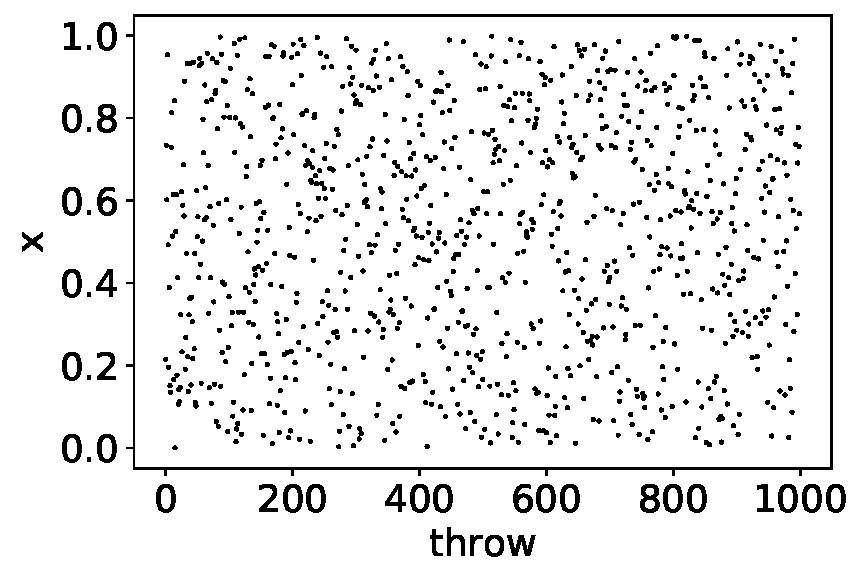
\includegraphics[height=0.22\textheight]{figs/labs/monte_carlo/flat2d.pdf} &
  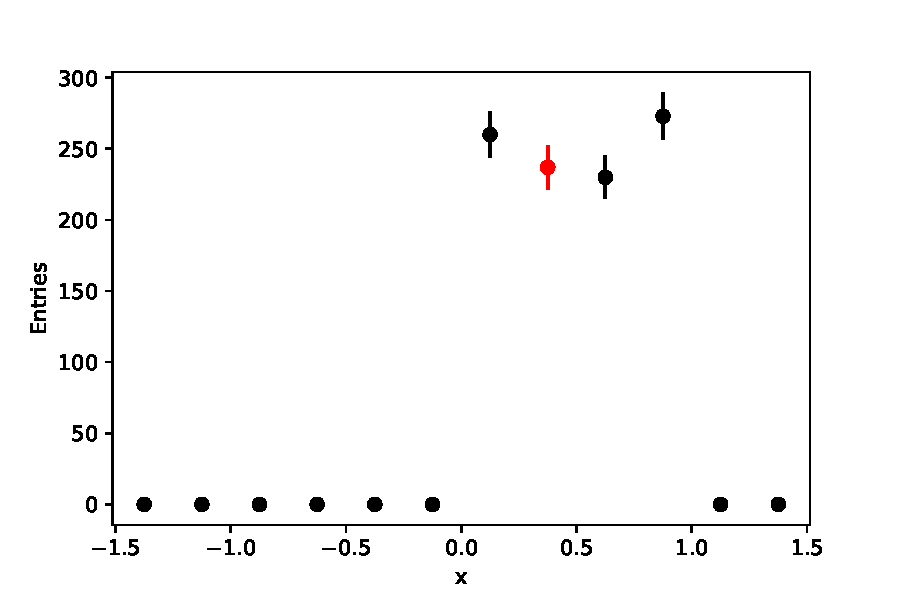
\includegraphics[height=0.22\textheight]{figs/labs/monte_carlo/flathist.pdf} \\
  (a) & (b) \\
 \end{tabular}
\caption{The (a) $x$ value of uniform random throws versus throw number and (b) corresponding histogram. }
\label{fig:flathist}
\end{center}
\end{figure}

\noindent
How can we verify that our Park-Miller random number generator
produces uniform random numbers in the range 0 to 1?  The associated
PDF is just $p(x)=1$, which we know how to plot, but how can we
compare this function to a sequence of numbers like $[0.21, 0.85,
  0.33, ...]$?  An initial attempt might look like
Fig.~\ref{fig:flathist}a, where we have simply plotted the $x$ value
of each throw versus the number of the throw.  Unfortunately, this
plot isn't particularly helpful.  If we zoomed in, we could determine
from the plot the $x$ value associated with each throw.  This is
simply too much information.

For interpreting a list of values as a distribution, there is only one
tool of choice: the histogram.  To histogram our data, we divide the
entire range $[0,1]$ into smaller ranges called {\em bins}.  Let's
start with 10 bins as an example. In this case, the first bin covers
the range from 0 to 0.1, or more precisely, the half-open interval
$\left[0,0.1\right)$ which includes $0$ and $0.099$, but not $0.1$.
  The second bin would have range $\left[0.1,0.2\right)$, the third
    bin would have range $\left[0.2,0.3\right)$ and so on, up to the
      last bin which would cover $\left[0.9,1.0\right]$.  To {\em
        fill} a histogram, you count the number of values that fall
      within the range of each bin.  So in our example, the value
      $0.21$ would add one to the count for the third bin, which has
      range $\left[0.2,0.3\right)$.  After filling, the histogram
        consists of a count associated with each bin range.

Fig.~\ref{fig:flathist}b shows a histogram filled with 1000 random
throws drawn from a uniform random number generator.  While we can now
see the shape of the distribution, we still don't have quite enough
information to answer the question, is this flat?  It is certainly not
perfectly flat!

The first feature we will need to add to the plot is the inclusion of
{\em error bars} to indicate the statistical uncertainty in our
histogram values.  Each histogram contains a {\em count} $n$ which
should follow a Poisson distribution with variance $\sigma^2 = n$.
Error bars are traditionally drawn with the size $\sigma$, which in
this case is $\sigma = \sqrt{n}$.  So when drawing a histogram, the
uncertainty in each bin is just the square root of the histogram
value.  That is the beauty of Poisson statistics!  If we have a count,
we know the statistical uncertainty.

\begin{figure}[htbp]
 \begin{center}
  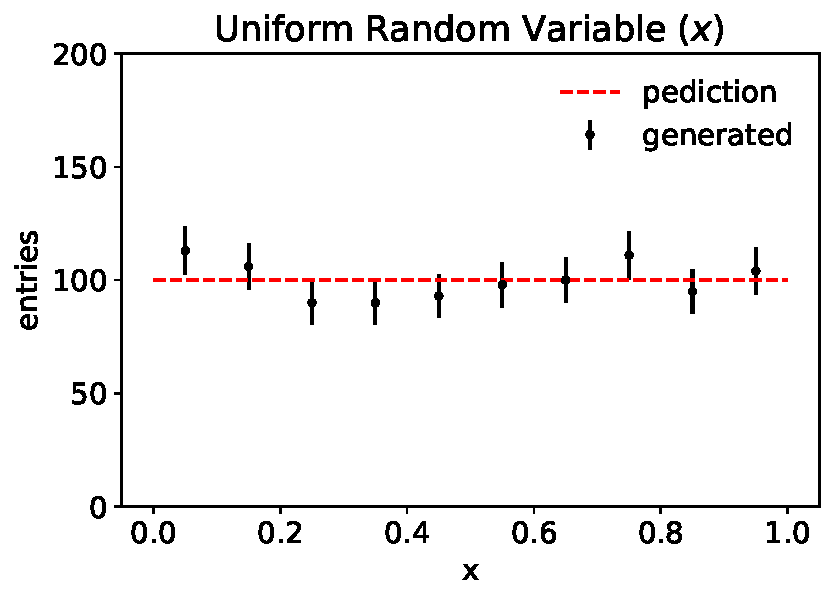
\includegraphics[width=0.50\textwidth]{figs/labs/monte_carlo/fancyhist.pdf}
  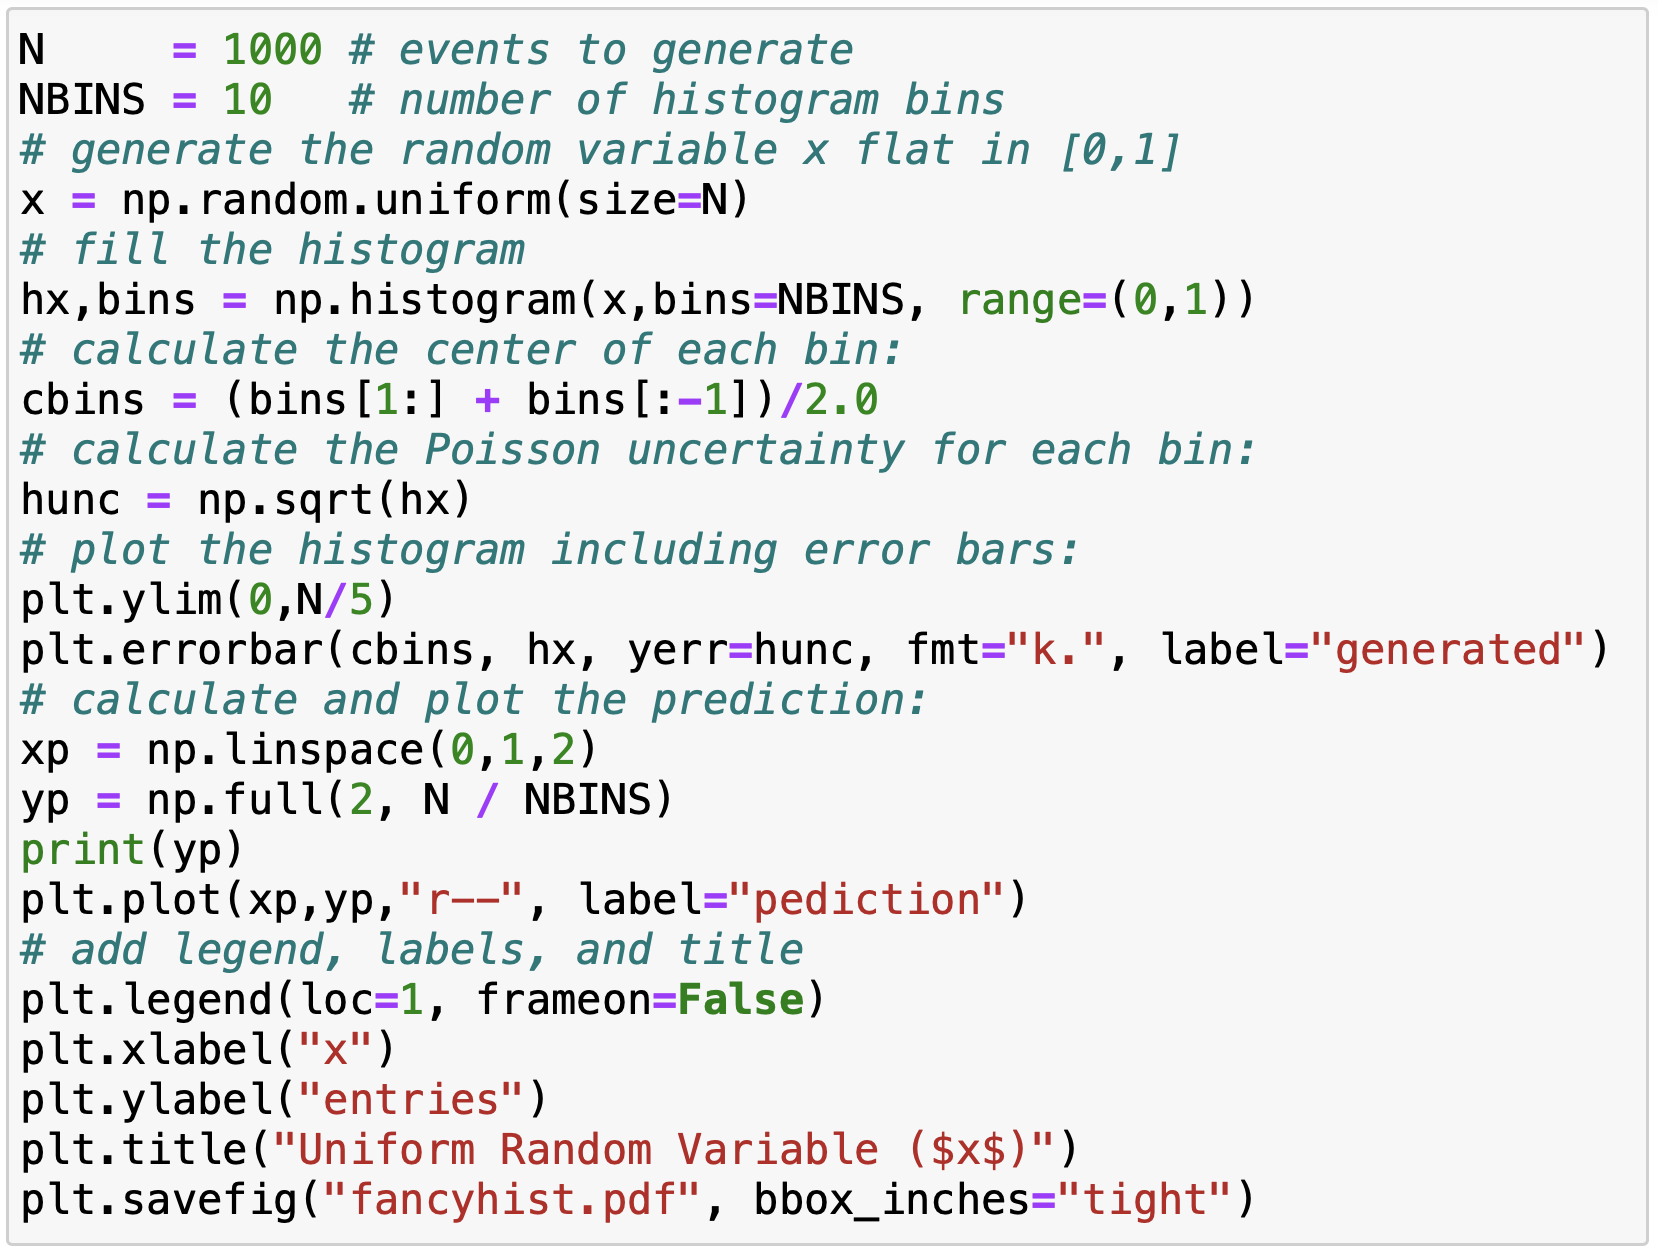
\includegraphics[width=0.75\textwidth]{figs/labs/monte_carlo/fancyhist-code.png}
\caption{Histogram of data drawn from a flat distribution compared to prediction, with the code used to produce the plot.}
\label{fig:fancyhist}
\end{center}
\end{figure}

We'll also want to add the prediction to the plot, assuming a flat
distribution for the contents of each bin.  In this case, we generated
$N$ events and we have $N_{\rm BINS}$ histogram bins, which should
therefore each contain an equal share: $N / N_{\rm BINS}$.  The
resulting histogram, along with the code used to generate it, is shown
in Fig.~\ref{fig:fancyhist}.  With the prediction and errorbars
included in the plot, one can now see that these generated values are
indeed quite consistent with a flat prediction. All of the bins are
within nearly one-sigma. With this number of bins, it is not uncommon
to see a two-sigma descrepancy.

You will produce many histograms in this class, so you will need to
(eventually) understand every single line in this example code.  Take
the time to read through the documentation for the key functions like
{\tt np.histogram} and {\tt np.random.uniform}, available on the web
(see numpy.org or just search ``np.histrogram python'').  A big part
of learning to program effectively, is learning how to read and
understand software documentation correctly and efficiently.

There are a few important features to notice:
\begin{itemize}
 \item The $x$-values are contained in an {\tt np.array} filled with
   uniform random variables generated by calling the {\tt
     np.random.uniform} function.
 \item The function {\tt np.histogram} is used to calculate a histogram
   from these $x$ values.  The call requests {\tt NBINS=10} histogram
   bins, in range $[0,1]$.  Don't confuse the python tuple {\tt (0,1)}
   used to indicate this range as indicating an open interval... often
   the computing language differs significantly from math notation, as
   is the case here!
 \item The {\tt np.histogram} function returns two items we need:  a {\tt np.array} containing the count for each bin ({\tt hx}) and a {\tt np.array} of bin edges ({\tt bins})
 \item We want to plot the count over the center of each bin, not one of the edges, so we calculate the quantity {\tt cbins} which is an {\tt np.array} containing the center of each bin.  You'll use this trick a lot, so make sure you understand what it is doing!
 \item The uncertainty on each bin {\tt hunc} is calculated as the square root of the bin counts {\tt hx}.
 \item We use the somewhat poorly named {\tt np.errorbar} function to plot {\bf both} the histogram central value {\tt and} the errorbar in each bin.
 \item We draw the prediction as a straight line defined by two points defined by {\tt xp} and {\tt yp}.
\end{itemize}

\begin{plot} \end{plot}
Modify the example code to generate a histogram for uniform random
numbers generated from your Park-Miller sequence instead of ${\tt
  np.random.uniform}$.  Increase the number of events to {\tt
  N=10000}.  Increase the number of bins to {\tt NBINS=20}.  Does your
code appear to produce uniform random numbers?

To answer a question in your notebook, simply add a cell and answer the question as a comment (each line starting with {\tt \#}).

\section{Calculating the value of $\pi$}

\begin{figure}[htbp]
\begin{center}
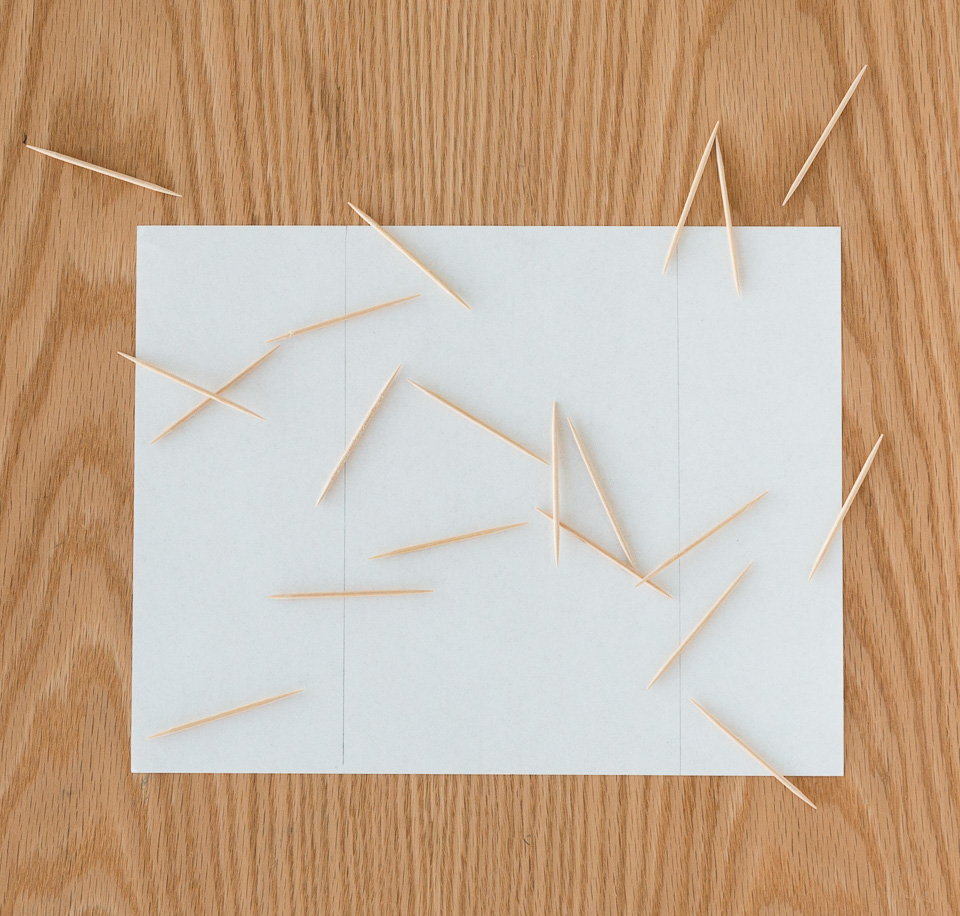
\includegraphics[width=0.65\textwidth]{figs/labs/monte_carlo/pitoss.jpg} 
\caption{Determining $\pi$ by throwing toothpicks.}
\label{fig:pitoss}
\end{center}
\end{figure}

\noindent
Hopefully 2021 will see the return of parties, so let's start by
examing a surefire way to be the life of the party: determining the
constant $\pi$ by throwing toothpicks!  The procedure is simple: you
cut a peice of paper to a width of four toothpicks, then draw two
vertical lines separated by the width of two tooth picks.  Take turns
tossing toothpicks, as in Fig.~\ref{fig:pitoss}.

From the geometry of the setup, it can be shown that the probability
that a toothpick which is entirely on the paper also crosses a line is
given by $1/\pi$.  Therefore, one can measure $\pi$ by counting the
total number of toothpicks that landed entirely on the page and
dividing by the number of those toothpicks that crossed a line.  This
is, in essence, the Monte Carlo method.

\begin{figure}[htbp]
\begin{center}
  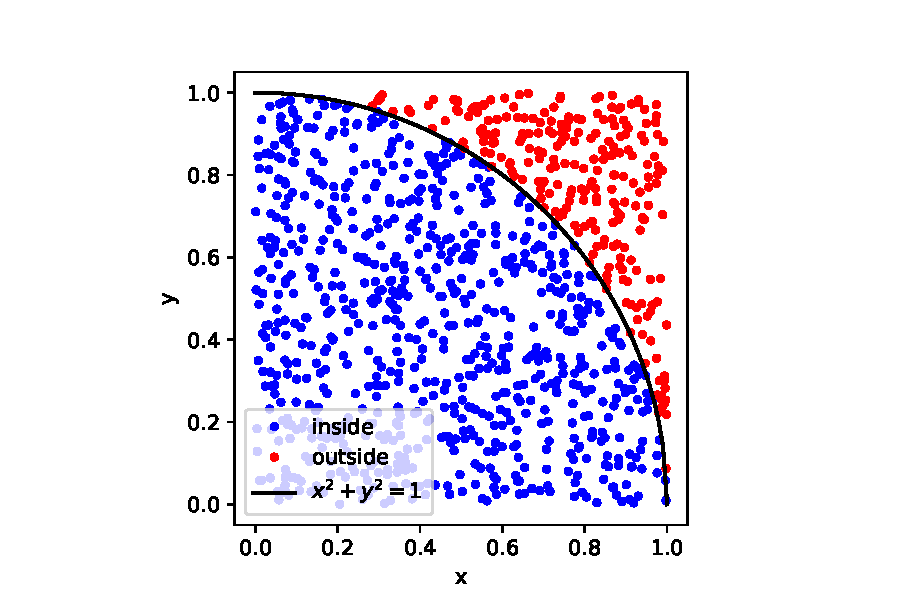
\includegraphics[width=0.50\textwidth]{figs/labs/monte_carlo/pimc.pdf}
  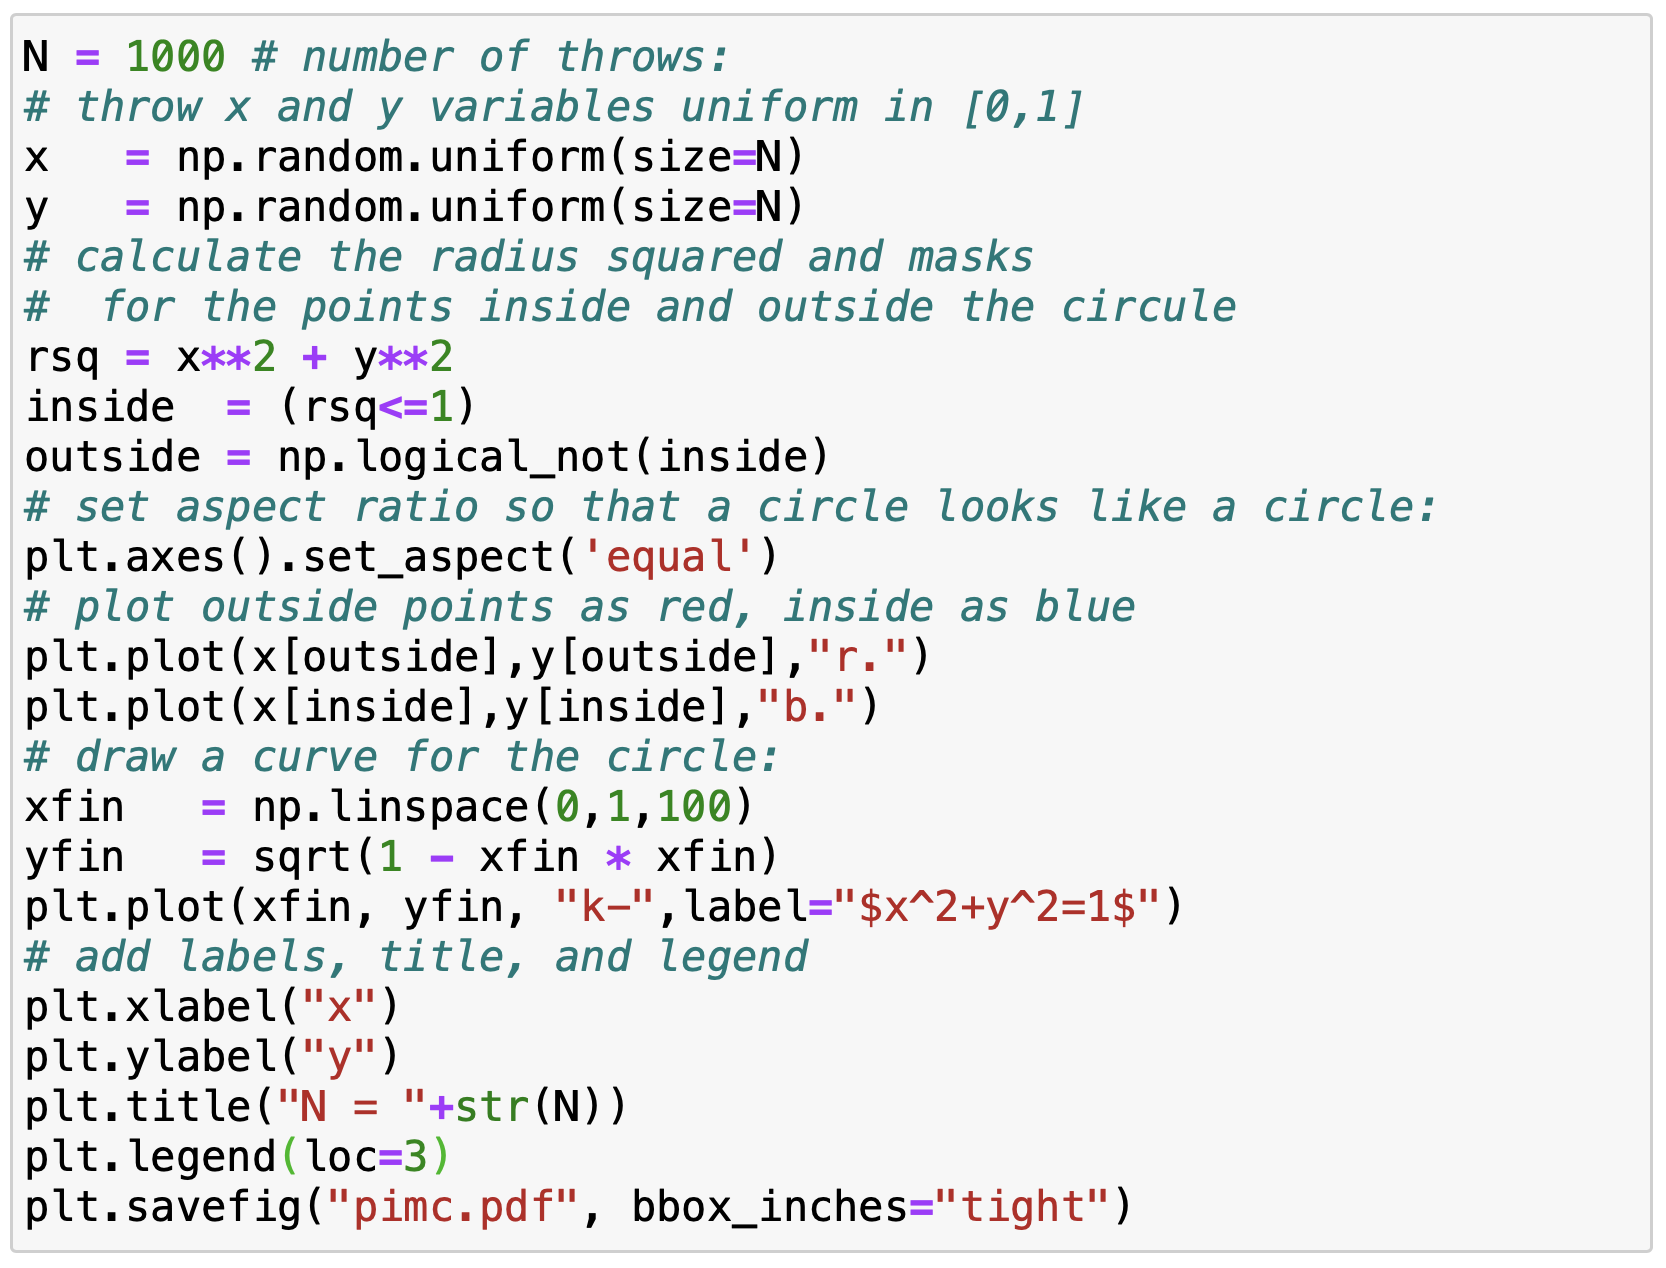
\includegraphics[width=0.75\textwidth]{figs/labs/monte_carlo/pimc-code.png} 
\caption{Monte Carlo Determination $\pi$ .}
\label{fig:pimc}
\end{center}
\end{figure}

An easier Monte Carlo method to implement computationally is shown in
Fig.~\ref{fig:pimc} along with the code used to generate the plot.
The idea is to throw points uniformly in the unit square of area 1.
Much like in the toothpick example, the value of $\pi$ can be
determined by counting the number of generated points that also landed
within the unit circle.

The key features of the example code are:
\begin{itemize}
\item The $x$ and $y$ values are each contained in an {\tt np.array} filled with uniform random variables in $[0,1]$ by the {\tt np.random.uniform} function.
\item A mask {\tt inside} is created to indicate which points are inside the circle.  Recall that the mask is an {\tt np.array} of True or False values, with the same length as the $x$ and $y$ arrays.  For example {\tt x[inside]} is an np.array containing just the subset of {\tt x} which are inside the circle.  
\end{itemize}

\begin{plot} \end{plot}
Starting from the example code, determine the numerical value of $\pi$
using the Monte Carlo method.  The easiest way to obtain the count you
need is to apply the function {\tt np.sum} to an appropriate mask.
When counting a mask, each True is treated as a one, and each False is
treated as zero.  Work out the relationship between $\pi$ and the
fraction of events in the unit circle, and use your count to
numerically determine the value of $\pi$.  Increase the number of
generated events and confirm that your calculated value of $\pi$
approaches the known value.

\begin{plot} \end{plot}
This is an example of a binomial process, because points are either
inside or outside the circle. So we expect the number of events in the
circle to follow the binomial distribution with $\sigma^2 = n \epsilon
(1-\epsilon)$.  In this case, $n$ is the total number of generated
events and $\epsilon$ is the fraction that fall inside the unit
circle.  The statistical uncertainty on your measured value of $\pi$
works out to be:
\begin{displaymath}
\sigma_\pi = \sqrt{\frac{\pi \, (4-\pi)}{n}}
\end{displaymath}
where $n$ is the number of generated events.  Does your measured value
of $\pi$ agree with the known value within your statistical
uncertainty?

\section{Monte Carlo integration}

The Monte Carlo method can also be used to numerically integrate a
function.  Monte Carlo integration methods generally only outperform
deterministic methods when the number of dimensions is large, but we
can illustrate the method most easily in one dimension. In this
section, you'll use the Monte Carlo method to perform the integral:
\begin{displaymath}
  \int_0^\pi \sin^2 \theta \, d\theta
\end{displaymath}

To do so, you should make a copy of your solution from the previous section
and modify it in the following manner:
\begin{itemize}
 \item Instead of thowing $x$ in $[0,1]$, throw $\theta$ in $[0,\pi]$.  This means the area of the rectangle $A$ is now $\pi$ instead of 1.
 \item Count the number of throws that land below the integral $y < \sin^2 \theta$.
 \item Determine the area under the curve as the fraction of the throws under the curve times the total area of the rectangle $A$.
 \item The statistical uncertainty in this case is $\pi/(2\sqrt{n})$ where $n$ is the number of generated events.
\end{itemize}  

\begin{plot} \end{plot}
Use the Monte Carlo method to calculate the integral:
\begin{displaymath}
  \int_0^\pi \sin^2 \theta \, d\theta
\end{displaymath}
Make a plot similar to that of Fig.~\ref{fig:pimc} showing the thows
above the curve in red and below the curve in blue.  Calculate the
integral and statistical uncertainty and compare it to the value you obtain analytically.

\section{The Rejection method}

\begin{figure}[htbp]
\begin{center}
  \begin{tabular}{cc}
  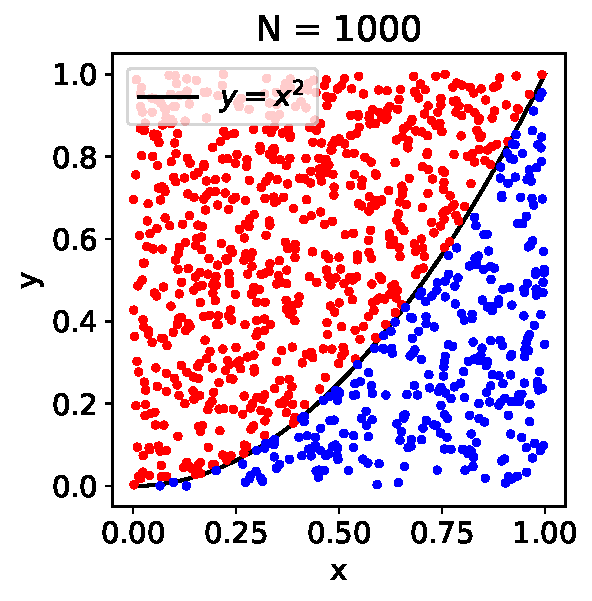
\includegraphics[height=0.30\textheight]{figs/labs/monte_carlo/rejectmc.pdf} &
  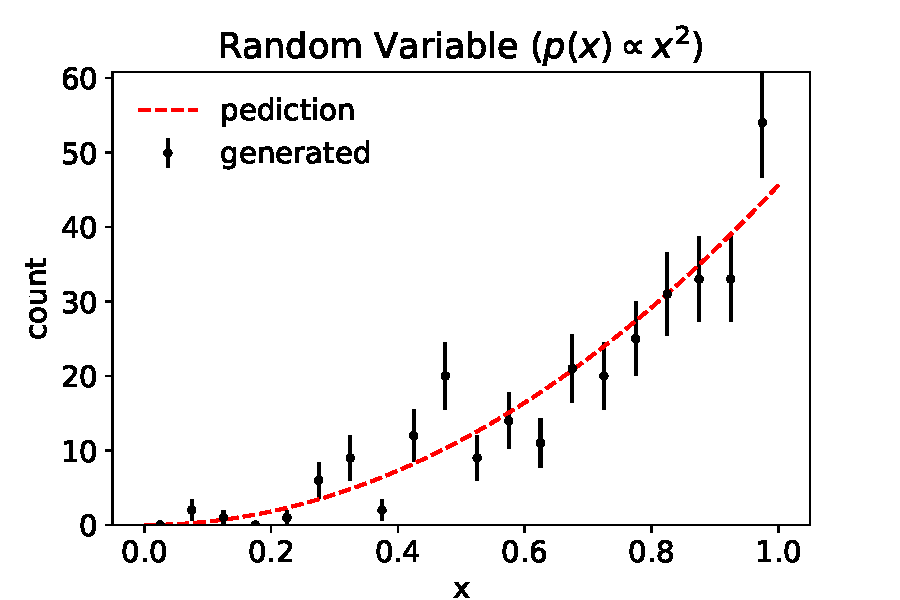
\includegraphics[height=0.30\textheight]{figs/labs/monte_carlo/quadhist.pdf} \\
  (a) & (b) \\
 \end{tabular}
  \caption{Monte Carlo rejection method applied to $p(x) \propto
    x^2$. Uniformly generated points (a) are rejected (red) if they
    are above the PDF, and the $x$ values of points below the PDF
    (blue) are selected.  A histogram (b) of the selected $x$ values
    shows that they follow the PDF.}
  \label{fig:rejectmc}
\end{center}
\end{figure}

\noindent
We now know how to generate uniform random numbers, but suppose we
need a random variable thrown according to a non-uniform probability
distribution $p(x)$?  Fig.~\ref{fig:rejectmc} demonstrates one
approach, which closely follows the procedure for numerical
integration using the Monte Carlo technique.

The rejection method produces random variables in a range from 0 to $L$
according to any desired PDF $p(x)$.  Start by finding a value $Y$ which is at
least as large as the maximum value of $p(x)$ for $x$ in $[0,L]$.  Then:
\begin{itemize}
  \item Throw $x$ as a uniform random variable in range $[0, L]$.
  \item Throw $y$ as a uniform random variable in range $[0, Y]$.
  \item If $y > p(x)$ reject the $x$ value and start over, otherwise, use the $x$ value as one throw.
\end{itemize}
Repeat these steps as necessary until a sufficent number of $x$ values have been selected.

The rejection method works because the probability of an $x$ value
being selected is, by construction, proportional to $p(x)$.  Since the
$x$ values were initially chosen from a flat distribution, the
selected $x$ values will follow the $p(x)$ distribution.  You can
visualize this in Fig.~\ref{fig:rejectmc} which leaves very little
doubt that the $x$ values of the blue points will follow the PDF.
Notice that it isn't even necessary for $p(x)$ to be normalized for
this procedure to work: any function proportional to the PDF of interest will do.

To produce a smooth function such as the quadratic prediction of
Fig.~\ref{fig:rejectmc}b, make sure you use plenty of $x$ values
(around 100 at least), via {\tt np.arange} or {\tt np.linspace}, just
as you did in the Plotting lab.  When comparing a PDF to histogrammed
data (as you will do for the second plot below) you will need to
normalize it appropriately.  The number of throws we expect to find in
a bin with edges at $a$ and $b$ is given by
\begin{displaymath}
  N \cdot \int_a^b p(x) \, dx \; = N \cdot p(x^*) \cdot (b-a) 
\end{displaymath}
The integral is simply the probability that one throw ends up in the
range, which we scale by the total number of throws $N$.  The equality
holds for at least one $x^*$ in the range $[a,b]$ and $(b-a)$ is
simply the bin size.  Therefore, we can formulate a prediction from a
normalized PDF $p(x)$ to data from $N$ throws used to fill a histogram with
bin sizes $\Delta x$ as the smooth function resulting from:
\begin{displaymath}
N \cdot p(x) \cdot \Delta x
\end{displaymath}
This is a technique we will use over and over again, so make sure you
understand it!

\begin{plot} \end{plot}
Use the rejection method to generate random numbers in the region from [0,1] that follow a distribution $p(x) \propto x^2$.  You'll do the following:
\begin{itemize}
  \item Note that there is no need to normalize the PDF when using the rejection method, so use $p(x)=x^2$.
  \item In our $x$ range $[0,1]$, $p(x)$ has maximum value at $x=1$ so set $Y = p(1) = 1^2 = 1$. 
  \item Throw $x$ as a uniform random variable in the range $[0, 1]$.
  \item As $Y=1$, throw $y$ as a uniform random variable in range $[0, 1]$.
  \item If $y > x^2$ reject the $x$ value and try a new set of $x$ and $y$ values, otherwise, use the $x$ value as one throw.
\end{itemize}
Throw 1000 (unselected) $x$ values, and produce a plot like that of
Fig.~\ref{fig:rejectmc}a showing your selected points in blue, your
rejected points in red, and the selection function ($p(x) = x^2$).

\begin{samepage}
\begin{plot} \end{plot}
Increase the number of (unselected) $x$ values thrown to 10,000.
Count the number $N$ of selected $x$ values.  Generate a plot like that of
Fig.~\ref{fig:rejectmc}b comparing the distribution of your selected
$x$ values to the prediction, which in this case is given by:
\begin{displaymath}
N \cdot 3x^2 \cdot \Delta x
\end{displaymath}
Be careful to use the number of selected $x$ values for $N$, not the total thrown (10000) before rejection.
\end{samepage}

\section{The transformation method}

Suppose that you need to throw random variables according to an
exponential distribution $p(x) = \exp(-x)$.  This PDF is defined for
$[0,+\infty)$ and properly normalized across this range as you can verify:
\begin{displaymath}
  \int_0^{+\infty} \exp(-x) \, dx = 1
\end{displaymath}    
The first problem is that we can only generate uniform random
variables up to a finite value $L$, not $+\infty$.  But let's suppose we are
willing to work aound this by simply cutting off the PDF at some large
value, like say we won't produce values with $x>100$.

With this change, the rejection method will work in principle.  But it
still has a major shortcoming.  Since $p(x)$ has a maximum value of 1,
and $x$ ranges from 0 to 100, the rectangle we will be filling with
uniform random points has area 100.  But our PDF, even when
integrated to $+\infty$, only has area 1.  So less than one out of
every 100 points we throw will be selected.  Perhaps we can live with
this, but then what if we need to go out to $x=1000000$.  Now only one
out of every million points will be selected.  In many scenarios, the
rejection method becomes too computationally inefficient to be of any
practical value.

In these case, we can use the transformation method instead of the
rejection method.  The transformation method is premised on the fact
that for {\em any} normalized PDF, we must have
\begin{displaymath}
  p(x) \geq 0
\end{displaymath}
everywhere and
\begin{displaymath}
  \int_{-\infty}^{+\infty} p(x) \; dx = 1
\end{displaymath}
as long as we take care to set $p(x)=0$ outside our range for $x$.  It follows from these properties that for any value of $y$ in the range $[0,1]$ there is a unique largest $x$ value for which:
\begin{equation} \label{eqn:mctransform}
  \int_{-\infty}^{x} p(x) \; dx = y
\end{equation}
From the fundamental theorem of calculus, we see that:
\begin{displaymath}
  dy = p(x) \, dx
\end{displaymath}
If the variables $y$ are drawn from a uniform distribution with PDF $q(y)=1$, then we see that:
\begin{displaymath}
 \int_{y_1}^{y_2} q(y) \, dy = \int_{x_1}^{x_2}p(x) \, dx.
\end{displaymath}
for $x_i$ and $y_i$ related by Eqn.~\ref{eqn:mctransform}.  This shows
that while $y$ is a uniform random variable ($q(y)=1$), the
corresponding $x$ values will distributed according to the desired PDF
$p(x)$.

That provides the mathematical justification for the transformation
method, which starts by finding the inverse function $f^{-1}(y)$ for:
\begin{displaymath}
  y = f(x) = \int_{-\infty}^{x} p(x) \, dx
\end{displaymath}
Then the procedure is:
\begin{itemize}  
 \item Throw $y$ as a uniform random variable in $[0,1]$.
 \item Find $x = f^{-1}(y)$
\end{itemize}
The $x$ values determined in this way will be drawn from the $p(x)$ distribution.  

There is an intuitive explanation for why this works.  The $y$ value is
essentially a fraction of the probability integrated by the PDF.  In a
region of $x$ where $p(x)$ is relatively large, the integral is
changing rapidly and so a large range of $y$ values map to this region
of $x$-values.  In a region of $x$ where $p(x)$ is relatively small,
the integral is not changing rapidly and so a small range of $y$
values map to this region of $x$-values.

Let's see how this applies to our exponential function.  In this case we calculate:
\begin{displaymath}
y = f(x) = \int_0^x \exp(-x) \, dx = 1 - \exp(-x)
\end{displaymath}  
which we invert to find:
\begin{displaymath}
x = - \ln(1-y)
\end{displaymath}  
To determine values of the random variable $x$, we follow this procedure:
\begin{itemize}
 \item Throw a $y$ value flat in [0,1]
 \item Caculate $x = -\ln(1-y)$
\end{itemize}
Repeat to produce as many $x$ values as needed.  Notice that this
procedure gives one usable $x$ value for every random throw.

\begin{plot} \end{plot}
Use the transformation method as described to generate 10,000 values
of a random variable thrown from an exponential function.  Produce a
plot like that of of Fig.~\ref{fig:rejectmc}b comparing the
distribution of your generated events to the prediction for $p(x) =
\exp(-x)$.  Remember to properly normalize your prediction based on
the bin size and number of events thrown.

\newpage
\section{Particle diffusion}

\begin{figure}[htbp]
\begin{center}
  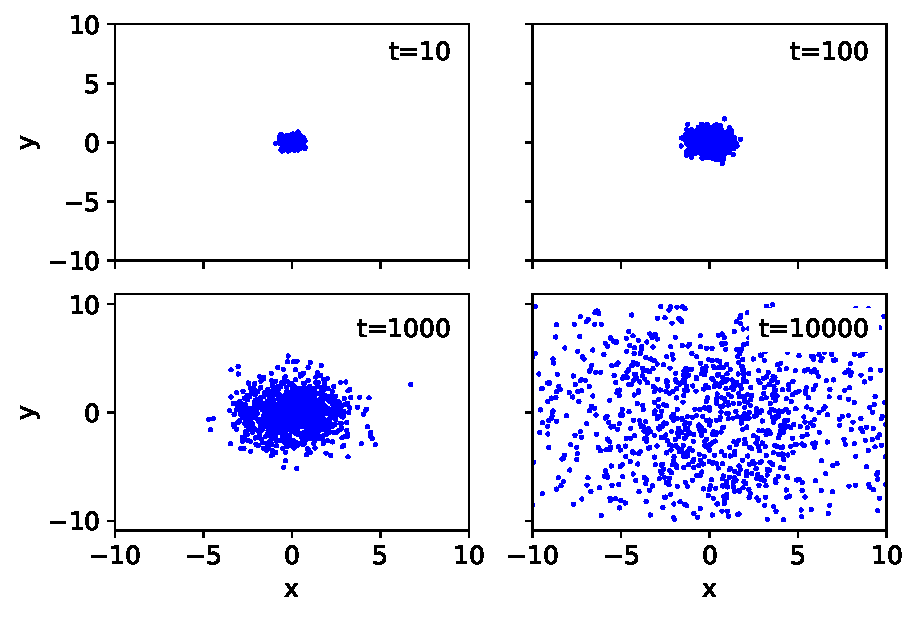
\includegraphics[width=0.80\textwidth]{figs/labs/monte_carlo/diffusion.pdf}
  \caption{Simulation of the diffusion of a drop of particles at four different times.}
\label{fig:diffusion}
\end{center}
\end{figure}

\begin{figure}[htbp]
 \begin{center}
  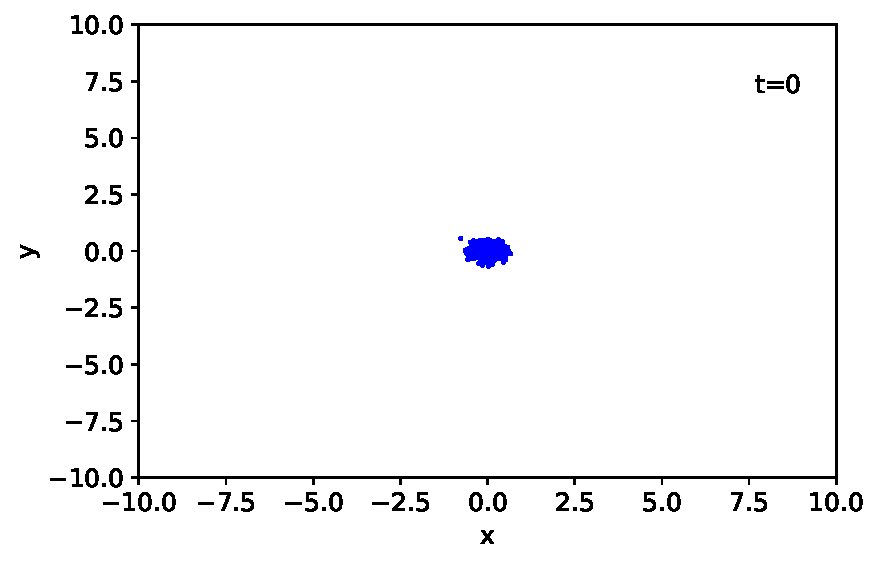
\includegraphics[width=0.50\textwidth]{figs/labs/monte_carlo/diffstart.pdf}
  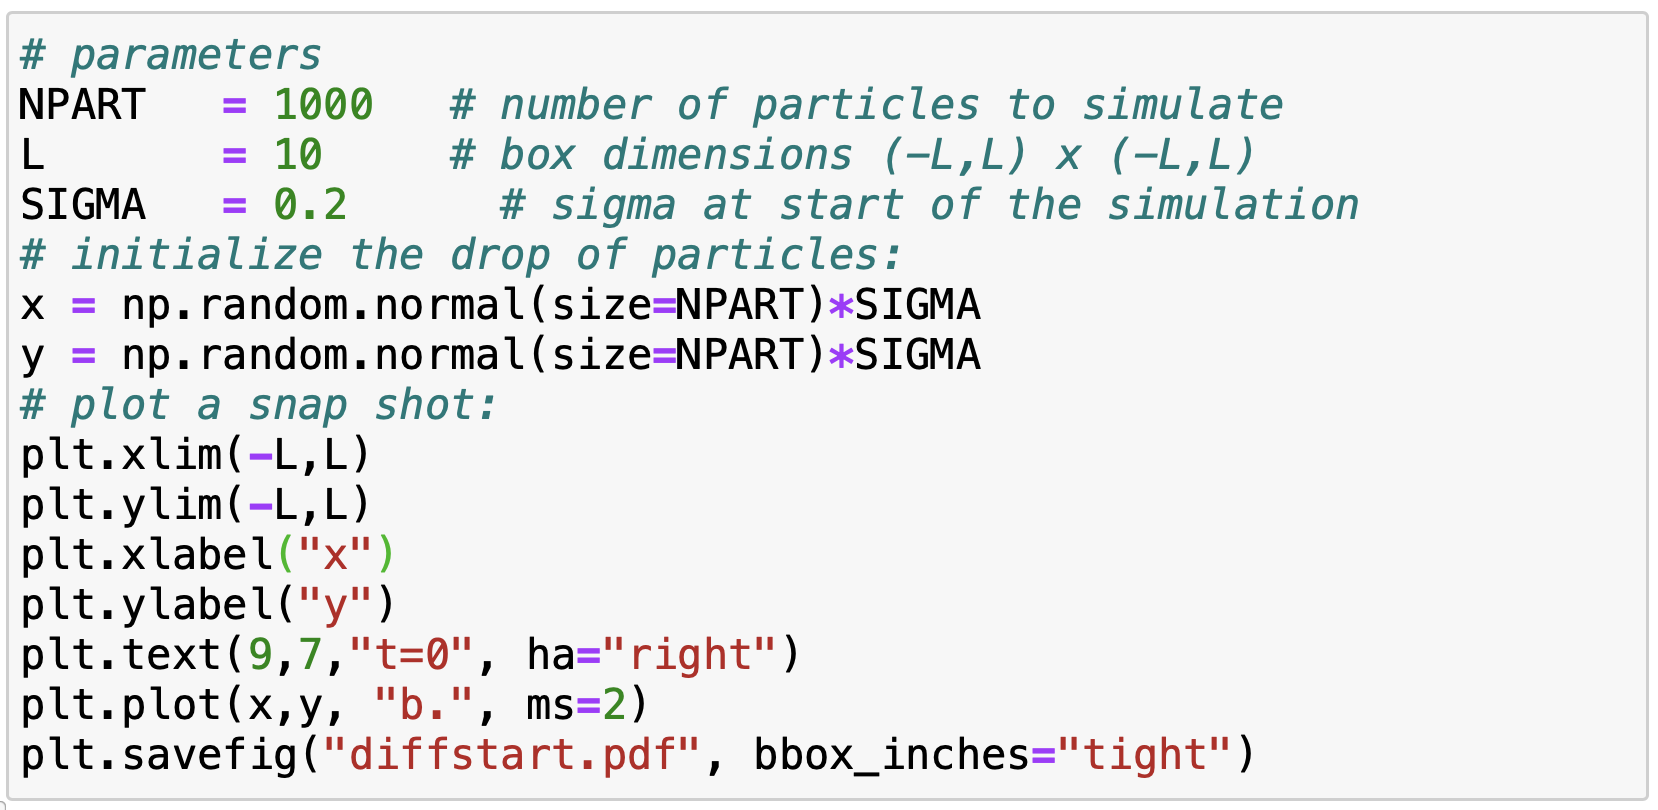
\includegraphics[width=0.75\textwidth]{figs/labs/monte_carlo/diffstart-code.png}
  \caption{Snapshot of the simulation at the start, along with the code used to produce it.}
\label{fig:diffstart}
\end{center}
\end{figure}


\noindent
In this section, we will model the diffusion of a drop of particles in
a medium, as in Fig.~\ref{fig:diffusion}, shown as snapshots at four
different times.  The starting point for the simulation, at $t=0$ is
shown in Fig.~\ref{fig:diffstart} along with the code used to produce
it.  The entire state of the system is contained in the arrays {\tt x}
and {\tt y} which contain the $x$ and $y$ positions of each particle.

The diffusion process is modeled by a random walk. During each update
(for one time step) the $x$ and $y$ values of each particle should be
randomly increased or decreased by an amount {\tt STEP=0.2} Any
particles that would leave the boundaries of the region $[-L,L]$ as a
result should be moved back into the region.  The numpy functions 
{\tt np.random.choice} and {\tt np.clip} are useful here.

Despite the symmetry of the random walk, the system clearly evolves by
diffusing outward over time.  This can be seen as a consequence of the
second law of thermodynamics.  Calculating the entropy from the
microscopic state of continuous particles is a bit tricky.  The
approach we will use is based on the Gibb's entropy.  We divide the
area into cells, and determine the fraction of the particles $f_i$ in
each cell $i$.  We calculate the entropy as:
\begin{displaymath}
  S = \sum_i f_i \ln f_i
\end{displaymath}
A python function which calculates the entropy in this manner:
\begin{tt}
\begin{verbatim}
from scipy import stats  
def entropy(x,y,l,sbins):
    h,xbins,ybins=np.histogram2d(x,y,bins=sbins,range=[[-l,l],[-l,l]])
    return stats.entropy(h.flatten())
\end{verbatim}
\end{tt}
The function takes as input parameters the position arrays {\tt x} and
{\tt y}, the boundary distance {\tt l} (set it to {\tt L} and the
number of bins in each dimension {\tt sbins} (set it to 20).  The
function returns the entropy of the current state of the system
described by {\tt x} and {\tt y}.

\begin{plot} \end{plot}
Starting from the example code, implement a random walk to model the
diffusion process, and plot four snap shops showing the evolution of
the system.

\begin{plot} \end{plot}
Calculate and record the entropy of the system as it evolves, and plot
the entropy as a function of time.


%\chapter{Simulation of an Ideal Gas}

\section{Introduction}

For an ideal gas composed of molecules with mass $m$ at temperature
$T$, the probability density for the component of velocity in the $x$
direction ($v_x$) is given by:
\begin{equation}
  \label{eqn:mbvx}
P(v_x) = \sqrt{\frac{m}{2 \pi k_{\rm B} T}} \exp\left(-\frac{m v_x^2}{2k_{\rm B} T}\right)
\end{equation}
where $k_{\rm B}$ is Boltzmann's constant.  Similary for the $y$ direction:
\begin{equation}
  \label{eqn:mbvx}
P(v_y) = \sqrt{\frac{m}{2 \pi k_{\rm B} T}} \exp\left(-\frac{m v_y^2}{2k_{\rm B} T}\right).
\end{equation}

For simplicity, we will be simulating a gas in two dimensions.  The infinitesimal probability associated with a velocity $(v_x, v_y)$ is given by: 
\begin{eqnarray*}
P(v_x, v_y) \, dv_x \, dv_y &=& P(v_x) \, dv_x \, P(v_y) \, dv_y \\
   &=& \frac{m}{2 \pi k_{\rm B} T} \exp\left(-\frac{m (v_x^2+v_y^2)}{2k_{\rm B} T}\right) \, dv_x \, dv_y \\
   &=& \frac{m v}{2 \pi k_{\rm B} T} \exp\left(-\frac{m v^2}{2k_{\rm B} T}\right) \, d\theta \, dv \\
\end{eqnarray*}
where we have changed to polar coordinates $v$ and $\theta$ in the usual manner with area differential $dv_x \, dv_y = v \, dv \, d\theta$.  This allows us to read off the probability density in polar coordintes:
\begin{equation*}
P(v, \theta) = \frac{m v}{2 \pi k_{\rm B} T} \exp\left(-\frac{m v^2}{2k_{\rm B} T}\right) 
\end{equation*}
Integrating over all possible directions $\theta$, we obtain:
\begin{eqnarray}
P(v) &=& \int_0^{2\pi} P(v,\theta) d\theta \nonumber \\
     &=& \int_0^{2\pi} \frac{m v}{2 \pi k_{\rm B} T} \exp\left(-\frac{m v^2}{2k_{\rm B} T}\right) \nonumber \\
P(v) &=& \frac{m v}{k_{\rm B} T} \exp \left(-\frac{m v^2}{2k_{\rm B} T}\right) \label{eqn:mbv}\\
\nonumber
\end{eqnarray}
which is the Maxwell-Boltzmann distribution for an ideal gas in two
dimensions.  This is the probability density for a gas molecule to have speed
$v$.

In this lab, we will create a simple numerical simulation of an ideal
gas and verify that the velocity of the gas follows the
Maxwell-Boltzmann distribution.

\section{System of Units}

Choosing an effective system of units is essential for building a
well-behaved numerical simulation.  Consider the Maxwell-Boltzmann
distribution, which involves the following SI values:
\begin{itemize}
\item Boltzmann's constant: $k_{\rm B} = 1.38 \times 10^{-23}~\rm J/K$
\item Molecular masses: e.g. $N_2$ with $m =  4.65 \times 10^{-26}~ \rm kg$.
\item Temperature: e.g. room temperature $T = 293~\rm K$.
\end{itemize}
The smallest number greater than zero that a computer can represent
with a single-precision floating point number is approximately
$10^{-38}$. Representing the SI value of Boltzmann's constant at
$10^{-23}$ uses a large fraction of this precision before we even begin
our calculation.  Numerical algorithms using floating point numbers
work best when the values involved in the calculation are near one.

It is usually best, therefore, to devise an alternate system of units
for any numerical simulation which keeps the values of variables of
interest as near one as possible.  We will call this the numerical
system of units.

To start, we choose a reference temperature near the temperature
we would like to simluate, say $T_0 = 293~\rm K$.  All temperatures in
the simulation will be in units of this reference temperature.  So a
temperature {\tt T=1.2} in the program will be $1.2 \, T_0 = 352~\rm K$
in SI units.  Our model also includes mass, so we choose a reference
mass near the mass of the molecules we will be simulating, say $M_0 =
4.65 \times 10^{-26}~ \rm kg$.  A mass {\tt m=2.1} in our program would have
an SI value value of $2.1 M_0 = 9.8 \times 10^{-26}~ \rm kg$.

The physics we will simulate involves Boltzmann's constant $k_{\rm B}$
which will have a value of one in our program.  This sets the
reference energy from our reference temeperature.  For example, an
energy {\tt kT = 3} in our program will have an SI value of $k_{\rm B}
T = 3~k_B T_0 = 1.21 \times 10^{-20}~J$.  The reference energy and
reference mass together define a reference velocity:
\begin{displaymath}
V_0 = \sqrt{\frac{k_b T_0}{M_0}} = 295~ \rm m/s.  
\end{displaymath}  

The only time the actual values choosen for the numerical system of
units are needed is if you need to convert inputs in SI units to the
numerical system of units, or convert the results of your simulation
to SI units.  In this lab, we will specify all inputs and report all
results using the numerical system of units.  {\bf So there is no need for
specific values such as $M_0 = 2.32 \times 10^{-25}~\rm kg$ to appear
anywhere in your program.}  If such values do appear, outside of
comments, you are certainly making a mistake!

\begin{figure}[htbp]
\begin{center}
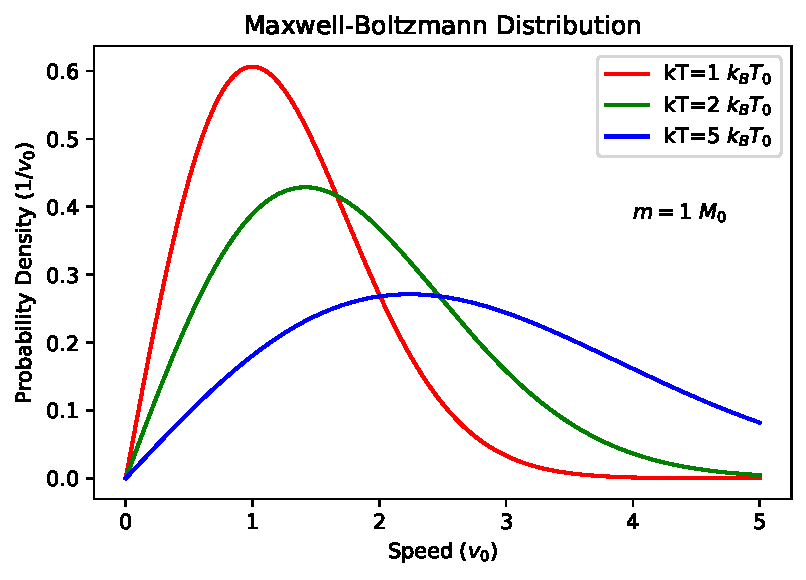
\includegraphics[width=0.65\textwidth]{figs/maxwellboltzman/maxboltz.pdf} \\
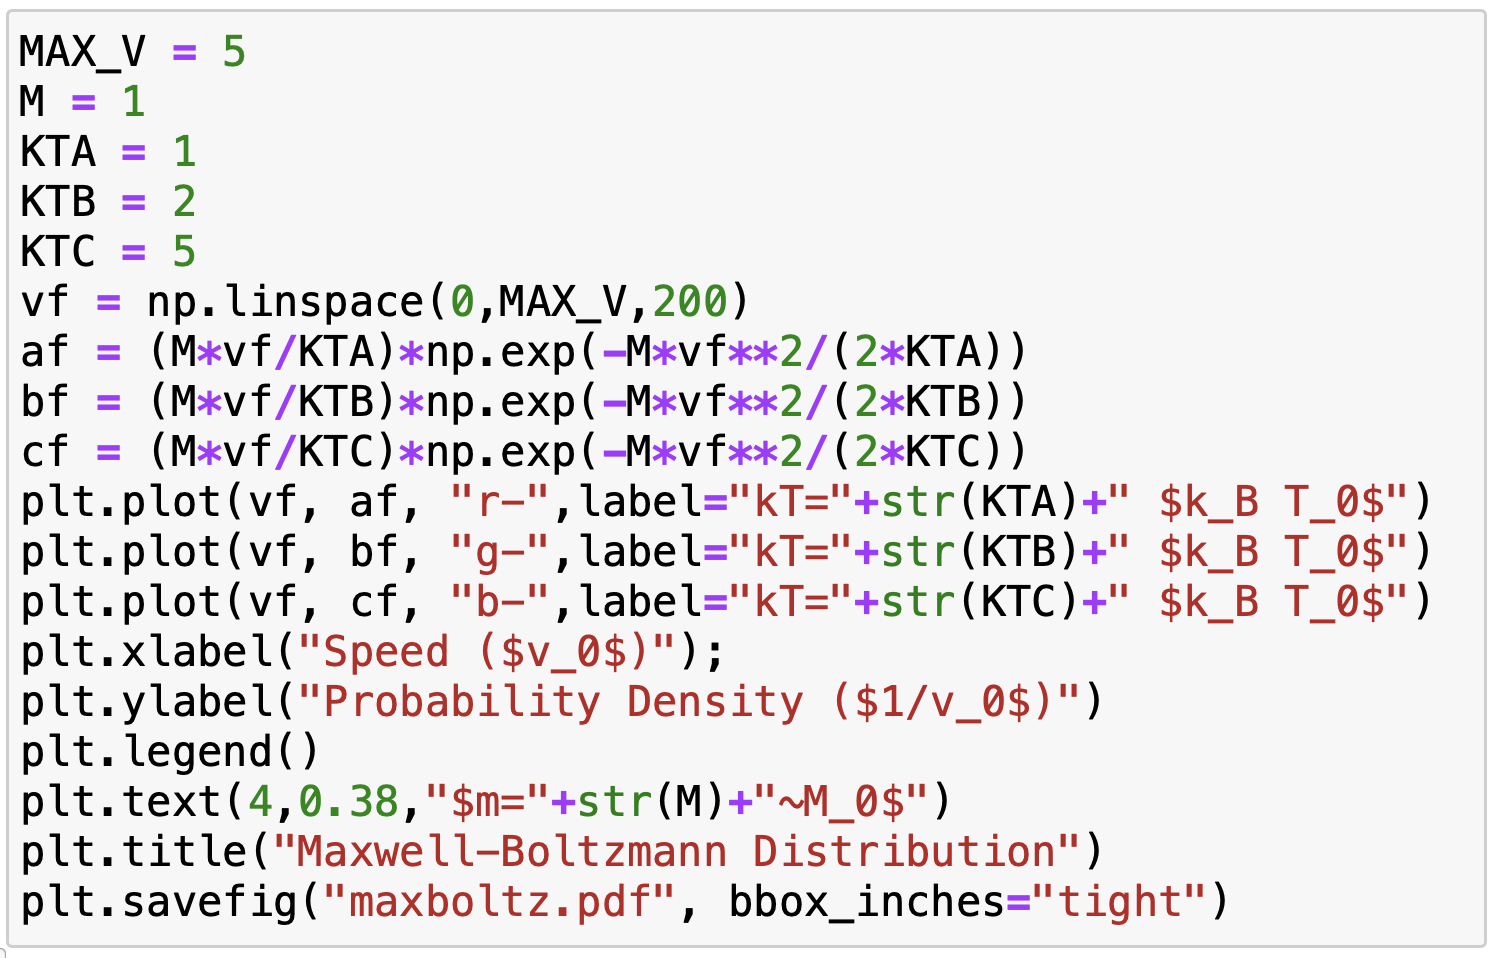
\includegraphics[width=0.65\textwidth]{figs/maxwellboltzman/maxboltz-code.png} \\
\caption{The Maxwell-Boltzmann distribution using a system of units appropriate for a numerical simulation, along with the code used to produce the plot.}
\label{fig:mbdist}
\end{center}
\end{figure}

As an example, the Maxwell-Boltzmann distribution is plotted in
Fig.~\ref{fig:mbdist} alongside the code used to produce it.  Notice
how for {\tt kT} and {\tt m} near one, the typical velcities are also
near one.  This is sign of good numerical system of units.  Notice
also that Boltzmann's constant or any other small or large numbers in
SI units do not appear anywhere in the code. 

\section{Collision Model}

At the heart of your numerical simulation is the collision model.  It
is the collisions of molecules that will allow your simulated gas to
reach thermal equilibrium.  We will use the simple elastic collision
of identical mass particles, as illustrated in Fig.~\ref{fig:collcms}, as our collision model.  We consider particles a and b with velocities $\vec{v_a}$ and
$\vec{v_b}$ in the lab frame.  The velocity of particle a in the CMS frame before the collision is
\begin{displaymath}
\vec{u} = \frac{\vec{v_a} - \vec{v_b}}{2}.
\end{displaymath}
The collision rotates the velocity of particle a by the scattering angle $\theta$ so that the velocity $\vec{w}$ after the collision is
\begin{displaymath}
\begin{pmatrix}
w_x \\
w_y \\
\end{pmatrix}
  =
\begin{pmatrix}
\cos \theta  & \sin \theta \\
-\sin \theta  & \cos \theta \\
\end{pmatrix}
\,
\begin{pmatrix}
u_x \\
u_y \\
\end{pmatrix}
\end{displaymath}
In the lab frame, the velocity of molecule a changes by an amount:
\begin{displaymath}
\Delta \vec{v_a} = \vec{w} - \vec{u}
\end{displaymath}
and the velocity of molecule b changes by an amount:
\begin{displaymath}
\Delta \vec{v_b} = \vec{u} - \vec{w}
\end{displaymath}




\begin{figure}[htbp]
\begin{center}
\begin{tikzpicture}
\draw[->, line width=1.5, blue] (-3,0) -- (-0.1,0);
\draw[->, line width=1.5, blue] (3,0)  -- (0.1,0);
\draw[->, line width=1.5, red] (0,0) -- (3*0.50,3*0.86) coordinate(A);
\draw[->, line width=1.5, red] (0,0) -- (-3*0.50,-3*0.86) coordinate(B);
\node[right] at (0.5,0.5) {$\theta$};
\node[left] at (-3,0) {a};
\node[right] at (3,0) {b};
\node[above] at (A) {a};
\node[below] at (B) {b};
\node[above] at (-1.5,0) {$\vec{u}$};
\node[above] at (1.5,0) {$-\vec{u}$};
\node[left] at (0.8,1.5) {$\vec{w}$};
\node[left] at (-0.8,-1.4) {$-\vec{w}$};
\end{tikzpicture}
\caption{The collision model in the center-of-mass:  incoming molecule $a$ with velocity $\vec{u}$ collides with the incoming particle $b$ of identical mass with velocity $-\vec{u}$.  Particle $a$ is scattered by angle $\theta$ and leaves with velocity $\vec{w}$, while particle $b$ leaves with velocity $\vec{w}$.  The magnitude of the final and initial velocities are the same:  $|\vec{u}| = |\vec{w}|$.}
\label{fig:collcms}
\end{center}
\end{figure}

\section{Implementing the Collision Model}

Our Python implementation for the collision will be computed in terms
of the components of the velocity vectors of molecule a and molecule
b:
\begin{eqnarray*}
\vec{v_a} &=& 
\begin{pmatrix}
a_x \\
a_y \\
\end{pmatrix} \\
\vec{v_b} &=& 
\begin{pmatrix}
b_x \\
b_y \\
\end{pmatrix} \\
\end{eqnarray*}
We'll use the Python variable names {\tt ax}, {\tt ay}, {\tt bx}, and {\tt by} to refer to $a_x$,  $a_y$,  $b_x$, and $b_y$.  

First calculate the $x$ and $y$ component of $\vec{u}$ as:
\begin{eqnarray*}
u_x &\equiv& \frac{a_x - b_x}{2} \\
u_y &\equiv& \frac{a_y - b_y}{2} \\
\end{eqnarray*}
Then compute the $x$ and $y$ component to the change in velocity of particle a and particle b:
\begin{eqnarray*}
  \Delta a_x &=& (\cos\theta - 1) \, u_x + \sin\theta \, u_y \\
  \Delta a_y &=& (\cos\theta - 1) \, u_y - \sin\theta \,  u_x \\
  \Delta b_x &=& (1-\cos\theta) \, u_x - \sin\theta \, u_y \\
  \Delta b_y &=& (1-\cos\theta) \, u_y + \sin\theta \,  u_x \\
\end{eqnarray*}
Finally, update the $x$ and $y$ components of the particle velocities to their value after the collision:
\begin{eqnarray*}
  a_x &\to& a_x + \Delta a_x \\
  a_y &\to& a_y + \Delta a_y \\
  b_x &\to& b_x + \Delta b_x \\
  b_y &\to& b_y + \Delta b_y \\
\end{eqnarray*}

In essential technique for programming complicated task is dividing
complicated tasks into smaller tasks, and thoroughly testing the
smaller tasks.  You cannot program effectively until you master this
technique.  I've taught students programming for many years, and the
students that finish last are invariably the ones that rush to
complete their entire program and then try to test and debug it.  This
approach always fails because when you do not get the right answer,
and you won't, ever, on the first try, you have absolutely no idea
what part of a very long chain of calculations is not programmed
correctly.

\begin{figure}[htbp]
\begin{center}
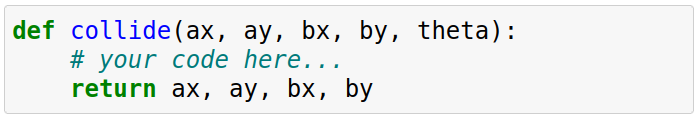
\includegraphics[width=0.65\textwidth]{figs/maxwellboltzman/collide.png} \\
\caption{Collision function.}
\label{fig:collfunc}
\end{center}
\end{figure}


To use this approach in the lab, we'll be implementing the collision
algorithm as a function, exactly as in Fig.~\ref{fig:collfunc}.  This
function takes as input the velocity components {\tt ax}, {\tt ay},
{\tt bx}, {\tt by} as defined above plus the scattering angle {\tt
  theta}.  In Fig.~\ref{fig:collfunc}, the function simply returns the
velocity components unchanged.  You should modify the function to
implement the scattering algoirthm described above.

Normally at this point, you would have to devise your own test to
validate your code.  One technique, that would work here, is to
calculate a few examples and then compare your program output to what
you obtained with paper and pencil.  For this lab, I will provide some
specific example calculations for you to validate your collision function.

\begin{figure}[htbp]
\begin{center}
  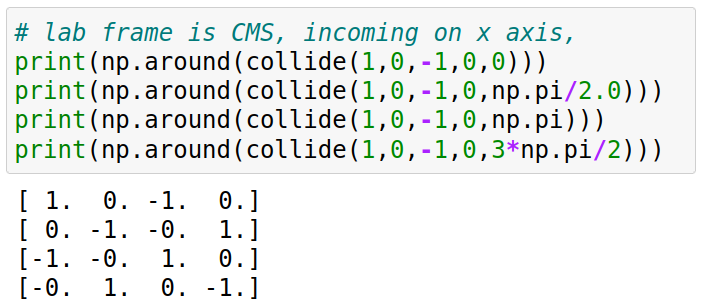
\includegraphics[width=0.65\textwidth]{figs/maxwellboltzman/collx.png} \\
  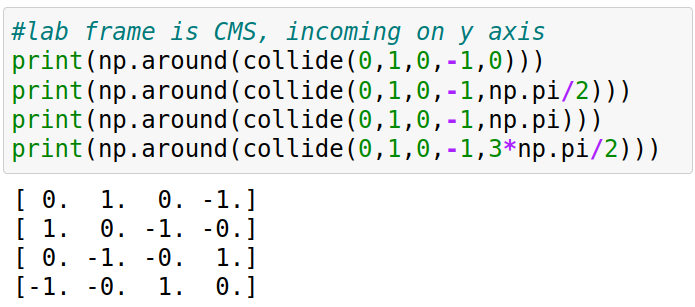
\includegraphics[width=0.65\textwidth]{figs/maxwellboltzman/colly.png} \\
  \caption{Example collisions along the $x$ and $y$ axis.}
\label{fig:collxy}
\end{center}
\end{figure}

\begin{plot} \end{plot}  Implement the collision algorithm as a function as in Fig.~\ref{fig:collfunc} and test it using example collisions from Fig.~\ref{fig:collxy}.

When testing your code, start with easy, special cases, such as used in Fig.~\ref{fig:collfunc}.  This helps makes it clearer where the program is failing.  Once your code works on the simple cases, escalate to more complicated examples.

\begin{figure}[htbp]
\begin{center}
  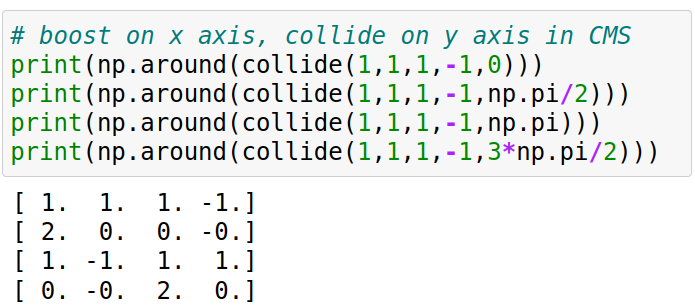
\includegraphics[width=0.65\textwidth]{figs/maxwellboltzman/collxy.png} \\
  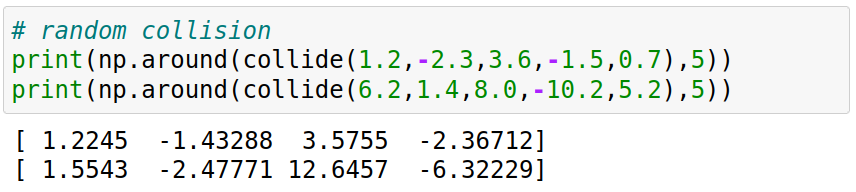
\includegraphics[width=0.65\textwidth]{figs/maxwellboltzman/collrand.png} \\
  \caption{More complicated example collisions.}
\label{fig:collcomp}
\end{center}
\end{figure}

\begin{plot} \end{plot}  Test your collision algorithm using the  example collisions from Fig.~\ref{fig:collcomp}.

\section{Initializing the Simulated Ideal Gas}

You will be modeling an ideal gas by direct Monte Carlo simulation of
{\tt NGAS} representative molecules.  We will use {\tt NGAS=1000}
intially, and you should use an even lower value while debugging.
We'll assume that the mass of each molecule in the gas is $M_0$,
or in the numerical system of units {\tt M=1}.

The state of your simulation will be completely contained in two numpy
arrays {\tt vx} and {\tt vy}, each of length {\tt NGAS}, which contain
the velocities of the particles in units of $V_0 = \sqrt{k_b T_0 /
  M_0}$.  Remember, the simulation uses a system of units that should
keep velocities near 1, so values such as 2.2, -3.1, 0.8, -0.01 are
all likely, and correspond to speeds up to several hundred meters per
second in SI units.  On the other hand, the presence of extremely
small values, like 5.3E-23, and extremely large values like 1.2E18 and
-8.2E28 are symptoms of bugs.

\begin{plot} Initialize both velocity arrays {\tt vx} and {\tt vy} of length {\tt NGAS}
with values choosen as uniform random variables in the range
$[-2,2]$. Fill two histograms, one with $v_x$ and one with $v_y$, with
an approriate range and 20 bins.  You should see that the velocities
are distributed uniformly (a flat distribution).  The distribution does not yet
resemble the Gaussian shape of Equation~\ref{eqn:mbvx} because it has not yet reached
thermal equilibrium.\end{plot}


\section{Collisions of an Ideal Gas}

To reach thermal equilibrium, you'll need to simulate collisions
betweens pairs of molecules in your gas.  For each collision, do the following:
\begin{itemize}
 \item Choose two molecules at random as particles $a$ and $b$. (See {\tt np.random.choice}.)
 \item Choose a random value $\theta$ uniformly in the range $[0,2\pi]$ (See {\tt np.random.uniform}.)
 \item Call your collision function with components of the velocity vectors for particles $a$ and $b$ and the scattering angle $\theta$.
 \item Update the velocity of particles $a$ and $b$ from the return value of your collision funciton
\end{itemize}   
For this model, you will need about 10 times as many collisions as gas
molecules in order to reach thermal equilibrium.

\begin{plot}  For {\tt NGAS=1000} simulate {\tt NCOLL = 10000} collisions as described above.
Fill two histograms, one with $v_x$ and one with $v_y$, with an
approriate range and 20 bins.  After reaching thermal equilibrium, the
distributions should resemble a Gaussian as predicted by Equation~\ref{eqn:mbvx}. \end{plot}

\section{Temperature of an Ideal Gas}

The temperature of the gas is related to the mean kinetic energy by:
\begin{equation}
\label{eqn:kt}
k_b T = m \, \frac{\braket{v_x^2} + \braket{v_y^2}}{2}  
\end{equation}  
You can estimate $\braket{v_x^2}$ from your simulation as {\tt np.mean(vx**2)}.

\begin{plot} Estimate $kT$ of the gas using Equation~\ref{eqn:kt} before and after simulating collisions.
The values should remain near the expected value 4/3.
\end{plot}

\section{The Maxwell-Boltzmann Distribution}

In this section, you'll reproduce the instructor plots of Fig.~\ref{fig:mbinst} using your own numerical simulation.

\begin{figure}[htbp]
\begin{center}
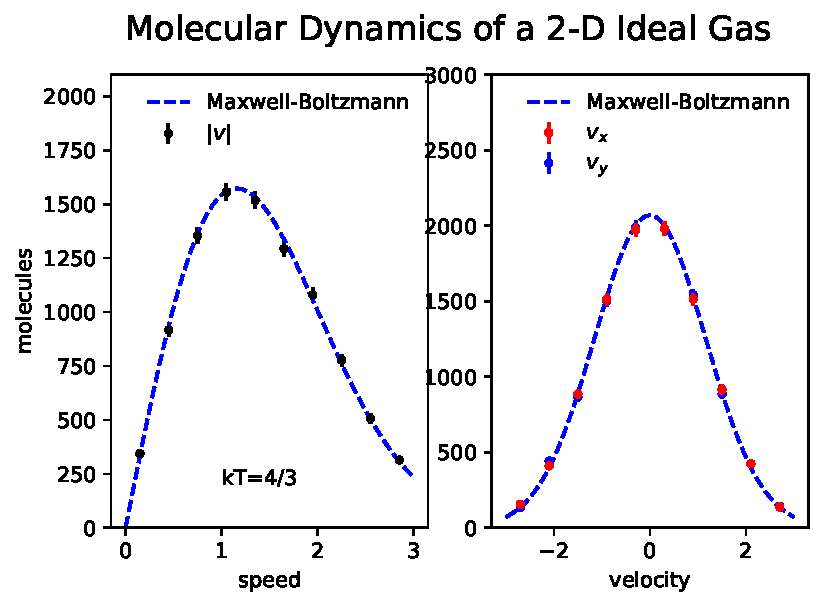
\includegraphics[width=0.85\textwidth]{figs/maxwellboltzman/maxboltz-instr.pdf} \\
\caption{Instructor plots.}
\label{fig:mbinst}
\end{center}
\end{figure}

\begin{plot}
  After your simulation reaches equilibrium, fill two histograms, one with $v_x$ and one with $v_y$, with an approriate range and 10 bins.  Compare with the prediction from Equation~\ref{eqn:mbvx}.  The results should resemble the right side of Fig.~\ref{fig:mbinst}, which were produced with {\tt NGAS=10000}.
\end{plot}

\begin{plot}
  After your simulation reaches equilibrium, fill a histograms with the magnitude of the velocity $v$, with an approriate range and 10 bins.  Compare with the prediction from Equation~\ref{eqn:mbv}.  The results should resemble the left side of Fig.~\ref{fig:mbinst}, which were produced with {\tt NGAS=10000}.
\end{plot}


  


\appendix

\chapter{Debugging}

In our context, debugging is the process of finding and removing
mistakes, called bugs, from your software.  Singling this process out
is a bit deceptive, it makes it seems distinct from software
development, as if you should write your software, and then debug it.
Indeed many students start this way, but it is a painful and
ineffective approach.  Experienced programs debug {\em while} developing
their code.

The fundamental approach to debugging (which works equally well
outside of programming) is to break every problem down into simple,
well defined parts, and then thoroughly test each part.  When one part
does not work, you break it down into smaller parts.  This process can
be quite simple, such as adding print statements to each step of a
complicated calculation.  It can also be quite advanced, such as when
teams of experienced software developers use automated builds and a
suite of integration tests that validate every proposed change to code
before it is accepted.  Experienced programs still produce bugs, they
just get better at squashing them.

There are a number of well-loved techniques to debugging:
\begin{itemize}
\item Print statements.
\item Start with a simple problem.
\item Test on special cases.
\item Use paper and pencil.
\item Decrease the size.
\item Establish feedback.
\item Write modular code.
\item Maintain unit tests.
\end{itemize}


\end{document}


